%%%%%%%%%%%%%%%%%%%%%%%%%%%%%%%%%%%%%%%%%
% Classicthesis Typographic Thesis
% LaTeX Template
% Version 1.0 (23/4/12)
%
% This template has been downloaded from:
% http://www.LaTeXTemplates.com
%
% Original author:
% Andr?Miede (http://www.miede.de)
%
% License:
% CC BY-NC-SA 3.0 (http://creativecommons.org/licenses/by-nc-sa/3.0/)
%
% General Tips:
% 1) Make sure to edit the classicthesis-config.file
% 2) New enumeration (A., B., C., etc in small caps): \begin{aenumerate} \end{aenumerate}
% 3) For margin notes: \marginpar or \graffito{}
% 4) Do not use bold fonts in this style, it is designed around them
% 5) Use tables as in the examples
% 6) See classicthesis-preamble.sty for useful commands
%
%%%%%%%%%%%%%%%%%%%%%%%%%%%%%%%%%%%%%%%%%

%----------------------------------------------------------------------------------------
%	PACKAGES AND OTHER DOCUMENT CONFIGURATIONS
%----------------------------------------------------------------------------------------
%
\documentclass[
		          twoside
		        , openright
		        , titlepage
		        , numbers = noenddot
		        , headinclude
		        %, headlines
		        , footinclude = true
		        , cleardoublepage = empty
		        , BCOR = 5mm
		        , paper = b5
		        , fontsize = 11pt
		        %, ngerman % Binding correction, paper type and font size
            , american % Languages
            , DIV = 12
              ]{scrreprt}
%\usepackage{CJK}
%%%%%%%%%%%%%%%%%%%%%%%%%%%%%%%%%%%%%%%%%
% Thesis Configuration File
%
% The main lines to change in this file are in the DOCUMENT VARIABLES
% section, the rest of the file is for advanced configuration.
%
%%%%%%%%%%%%%%%%%%%%%%%%%%%%%%%%%%%%%%%%%

%----------------------------------------------------------------------------------------
%	DOCUMENT VARIABLES
%	Fill in the lines below to enter your information into the thesis template
%	Each of the commands can be cited anywhere in the thesis
%----------------------------------------------------------------------------------------

% Remove drafting to get rid of the '[ Date - classicthesis version 4.0 ]' text at the bottom of every page
\PassOptionsToPackage{eulerchapternumbers, listings,drafting, pdfspacing, subfig,beramono,eulermath,parts}{style/classicthesis}
% Available options: drafting parts nochapters linedheaders eulerchapternumbers beramono eulermath pdfspacing minionprospacing tocaligned dottedtoc manychapters listings floatperchapter subfig
% Adding 'dottedtoc' will make page numbers in the table of contents flushed right with dots leading to them

\newcommand{\myTitle}{A Classic Thesis Style\xspace}
\newcommand{\mySubtitle}{An Homage to The Elements of Typographic Style\xspace}
\newcommand{\myDegree}{Doktor-Ingenieur (Dr.-Ing.)\xspace}
\newcommand{\myName}{Andr\'e Miede\xspace}
\newcommand{\myProf}{Put name here\xspace}
\newcommand{\myOtherProf}{Put name here\xspace}
\newcommand{\mySupervisor}{Put name here\xspace}
\newcommand{\myFaculty}{Put data here\xspace}
\newcommand{\myDepartment}{Put data here\xspace}
\newcommand{\myUni}{Put data here\xspace}
\newcommand{\myLocation}{Darmstadt\xspace}
\newcommand{\myTime}{December 2011\xspace}
\newcommand{\myVersion}{version 4.0\xspace}

%----------------------------------------------------------------------------------------
%	USEFUL COMMANDS
%----------------------------------------------------------------------------------------

\newcommand{\ie}{i.\,e.}
\newcommand{\Ie}{I.\,e.}
\newcommand{\eg}{e.\,g.}
\newcommand{\Eg}{E.\,g.}

\newcounter{dummy} % Necessary for correct hyperlinks (to index, bib, etc.)
\providecommand{\mLyX}{L\kern-.1667em\lower.25em\hbox{Y}\kern-.125emX\@}

%----------------------------------------------------------------------------------------
%	PACKAGES
%----------------------------------------------------------------------------------------
\usepackage{bm}
\usepackage[nohints]{minitoc}
\usepackage{nicefrac}
\usepackage{booktabs}
\usepackage{float}
\usepackage{lipsum}
\usepackage{amsthm}
\newtheorem{example}{Example}
% Used for inserting dummy 'Lorem ipsum' text into the template

%------------------------------------------------

\PassOptionsToPackage{latin9}{inputenc} % latin9 (ISO-8859-9) = latin1+"Euro sign"
\usepackage{inputenc}

 %------------------------------------------------

%\PassOptionsToPackage{ngerman,american}{babel}  % Change this to your language(s)
% Spanish languages need extra options in order to work with this template
%\PassOptionsToPackage{spanish,es-lcroman}{babel}
\usepackage{babel}

%------------------------------------------------

\PassOptionsToPackage{square,numbers}{natbib}
 \usepackage{natbib}

 %------------------------------------------------

\PassOptionsToPackage{fleqn}{amsmath} % Math environments and more by the AMS
 \usepackage{amsmath}

 %------------------------------------------------

\PassOptionsToPackage{T1}{fontenc} % T2A for cyrillics
\usepackage{fontenc}

%------------------------------------------------

\usepackage{xspace} % To get the spacing after macros right

%------------------------------------------------

\usepackage{mparhack} % To get marginpar right

%------------------------------------------------

\usepackage{fixltx2e} % Fixes some LaTeX stuff

%------------------------------------------------

\PassOptionsToPackage{smaller}{acronym} % Include printonlyused in the first bracket to only show acronyms used in the text
\usepackage{acronym} % nice macros for handling all acronyms in the thesis

%------------------------------------------------

%\renewcommand*{\acsfont}[1]{\textssc{#1}} % For MinionPro
%\renewcommand{\bflabel}[1]{{#1}\hfill} % Fix the list of acronyms

%------------------------------------------------

\PassOptionsToPackage{pdftex}{graphicx}
\usepackage{graphicx}

%----------------------------------------------------------------------------------------
%	FLOATS: TABLES, FIGURES AND CAPTIONS SETUP
%----------------------------------------------------------------------------------------

\usepackage{tabularx} % Better tables
\setlength{\extrarowheight}{3pt} % Increase table row height
\newcommand{\tableheadline}[1]{\multicolumn{1}{c}{\textsc{#1}}}
\newcommand{\myfloatalign}{\centering} % To be used with each float for alignment
\usepackage{caption}
\captionsetup{format=hang,font=small}
\usepackage{subfig}

\usepackage{longtable,booktabs}


%----------------------------------------------------------------------------------------
%	CODE LISTINGS SETUP
%----------------------------------------------------------------------------------------

\usepackage{listings}
%\lstset{emph={trueIndex,root},emphstyle=\color{BlueViolet}}%\underbar} % for special keywords
\lstset{language=[LaTeX]Tex, % Specify the language for listings here
keywordstyle=\color{RoyalBlue}, % Add \bfseries for bold
basicstyle=\small\ttfamily, % Makes listings a smaller font size and a different font
%identifierstyle=\color{NavyBlue}, % Color of text inside brackets
commentstyle=\color{Green}\ttfamily, % Color of comments
stringstyle=\rmfamily, % Font type to use for strings
numbers=left, % Change left to none to remove line numbers
numberstyle=\scriptsize, % Font size of the line numbers
stepnumber=5, % Increment of line numbers
numbersep=8pt, % Distance of line numbers from code listing
showstringspaces=false, % Sets whether spaces in strings should appear underlined
breaklines=true, % Force the code to stay in the confines of the listing box
%frameround=ftff, % Uncomment for rounded frame
frame=single, % Frame border - none/leftline/topline/bottomline/lines/single/shadowbox/L
belowcaptionskip=.75\baselineskip % Space after the "Listing #: Desciption" text and the listing box
}

%----------------------------------------------------------------------------------------
%	HYPERREFERENCES
%----------------------------------------------------------------------------------------

\PassOptionsToPackage{pdftex,hyperfootnotes=false,pdfpagelabels}{hyperref}
\usepackage{hyperref}  % backref linktocpage pagebackref
\pdfcompresslevel=9
\pdfadjustspacing=1

\hypersetup{
% Uncomment the line below to remove all links (to references, figures, tables, etc)
%draft,
colorlinks=true, linktocpage=true, pdfstartpage=3, pdfstartview=FitV,
% Uncomment the line below if you want to have black links (e.g. for printing black and white)
%colorlinks=false, linktocpage=false, pdfborder={0 0 0}, pdfstartpage=3, pdfstartview=FitV,
breaklinks=true, pdfpagemode=UseNone, pageanchor=true, pdfpagemode=UseOutlines,
plainpages=false, bookmarksnumbered, bookmarksopen=true, bookmarksopenlevel=1,
hypertexnames=true, pdfhighlight=/O, urlcolor=webbrown, linkcolor=RoyalBlue, citecolor=webgreen,
%------------------------------------------------
% PDF file meta-information
pdftitle={\myTitle},
pdfauthor={\textcopyright\ \myName, \myUni, \myFaculty},
pdfsubject={},
pdfkeywords={},
pdfcreator={pdfLaTeX},
pdfproducer={LaTeX with hyperref and classicthesis}
%------------------------------------------------
}

%----------------------------------------------------------------------------------------
%	BACKREFERENCES
%----------------------------------------------------------------------------------------

\usepackage{ifthen} % Allows the user of the \ifthenelse command
\newboolean{enable-backrefs} % Variable to enable backrefs in the bibliography
\setboolean{enable-backrefs}{false} % Variable value: true or false

\newcommand{\backrefnotcitedstring}{\relax} % (Not cited.)
\newcommand{\backrefcitedsinglestring}[1]{(Cited on page~#1.)}
\newcommand{\backrefcitedmultistring}[1]{(Cited on pages~#1.)}
\ifthenelse{\boolean{enable-backrefs}} % If backrefs were enabled
{
\PassOptionsToPackage{hyperpageref}{backref}
\usepackage{backref} % to be loaded after hyperref package
\renewcommand{\backreftwosep}{ and~} % separate 2 pages
\renewcommand{\backreflastsep}{, and~} % separate last of longer list
\renewcommand*{\backref}[1]{}  % disable standard
\renewcommand*{\backrefalt}[4]{% detailed backref
\ifcase #1
\backrefnotcitedstring
\or
\backrefcitedsinglestring{#2}
\else
\backrefcitedmultistring{#2}
\fi}
}{\relax}

%----------------------------------------------------------------------------------------
%	AUTOREFERENCES SETUP
%	Redefines how references in text are prefaced for different
%	languages (e.g. "Section 1.2" or "section 1.2")
%----------------------------------------------------------------------------------------

\makeatletter
\@ifpackageloaded{babel}
{
\addto\extrasamerican{
\renewcommand*{\figureautorefname}{Figure}
\renewcommand*{\tableautorefname}{Table}
\renewcommand*{\partautorefname}{Part}
\renewcommand*{\chapterautorefname}{Chapter}
\renewcommand*{\sectionautorefname}{Section}
\renewcommand*{\subsectionautorefname}{Section}
\renewcommand*{\subsubsectionautorefname}{Section}
}
\addto\extrasngerman{
\renewcommand*{\paragraphautorefname}{Absatz}
\renewcommand*{\subparagraphautorefname}{Unterabsatz}
\renewcommand*{\footnoteautorefname}{Fu\"snote}
\renewcommand*{\FancyVerbLineautorefname}{Zeile}
\renewcommand*{\theoremautorefname}{Theorem}
\renewcommand*{\appendixautorefname}{Anhang}
\renewcommand*{\equationautorefname}{Gleichung}
\renewcommand*{\itemautorefname}{Punkt}
}
\providecommand{\subfigureautorefname}{\figureautorefname} % Fix to getting autorefs for subfigures right
}{\relax}
\makeatother

%----------------------------------------------------------------------------------------

\usepackage{style/classicthesis}

%----------------------------------------------------------------------------------------
%	CHANGING TEXT AREA
%----------------------------------------------------------------------------------------

%\linespread{1.05} % a bit more for Palatino
%\areaset[current]{312pt}{761pt} % 686 (factor 2.2) + 33 head + 42 head \the\footskip
%\setlength{\marginparwidth}{7em}%
%\setlength{\marginparsep}{2em}%

%----------------------------------------------------------------------------------------
%	USING DIFFERENT FONTS
%----------------------------------------------------------------------------------------

%\usepackage[oldstylenums]{kpfonts} % oldstyle notextcomp
%\usepackage[osf]{libertine}
%\usepackage{hfoldsty} % Computer Modern with osf
%\usepackage[light,condensed,math]{iwona}
%\renewcommand{\sfdefault}{iwona}
%\usepackage{lmodern} % <-- no osf support :-(
%\usepackage[urw-garamond]{mathdesign} <-- no osf support :-(

\usepackage{color}
\usepackage{fancyvrb}
\newcommand{\VerbBar}{|}
\newcommand{\VERB}{\Verb[commandchars=\\\{\}]}
\DefineVerbatimEnvironment{Highlighting}{Verbatim}{commandchars=\\\{\}}
% Add ',fontsize=\small' for more characters per line

\usepackage{framed}
\definecolor{shadecolor}{RGB}{248,248,248}
\newenvironment{Shaded}{\begin{snugshade}}{\end{snugshade}}
\newcommand{\KeywordTok}[1]{\textcolor[rgb]{0.13,0.29,0.53}{\textbf{{#1}}}}
\newcommand{\DataTypeTok}[1]{\textcolor[rgb]{0.13,0.29,0.53}{{#1}}}
\newcommand{\DecValTok}[1]{\textcolor[rgb]{0.00,0.00,0.81}{{#1}}}
\newcommand{\BaseNTok}[1]{\textcolor[rgb]{0.00,0.00,0.81}{{#1}}}
\newcommand{\FloatTok}[1]{\textcolor[rgb]{0.00,0.00,0.81}{{#1}}}
\newcommand{\ConstantTok}[1]{\textcolor[rgb]{0.00,0.00,0.00}{{#1}}}
\newcommand{\CharTok}[1]{\textcolor[rgb]{0.31,0.60,0.02}{{#1}}}
\newcommand{\SpecialCharTok}[1]{\textcolor[rgb]{0.00,0.00,0.00}{{#1}}}
\newcommand{\StringTok}[1]{\textcolor[rgb]{0.31,0.60,0.02}{{#1}}}
\newcommand{\VerbatimStringTok}[1]{\textcolor[rgb]{0.31,0.60,0.02}{{#1}}}
\newcommand{\SpecialStringTok}[1]{\textcolor[rgb]{0.31,0.60,0.02}{{#1}}}
\newcommand{\ImportTok}[1]{{#1}}
\newcommand{\CommentTok}[1]{\textcolor[rgb]{0.56,0.35,0.01}{\textit{{#1}}}}
\newcommand{\DocumentationTok}[1]{\textcolor[rgb]{0.56,0.35,0.01}{\textbf{\textit{{#1}}}}}
\newcommand{\AnnotationTok}[1]{\textcolor[rgb]{0.56,0.35,0.01}{\textbf{\textit{{#1}}}}}
\newcommand{\CommentVarTok}[1]{\textcolor[rgb]{0.56,0.35,0.01}{\textbf{\textit{{#1}}}}}
\newcommand{\OtherTok}[1]{\textcolor[rgb]{0.56,0.35,0.01}{{#1}}}
\newcommand{\FunctionTok}[1]{\textcolor[rgb]{0.00,0.00,0.00}{{#1}}}
\newcommand{\VariableTok}[1]{\textcolor[rgb]{0.00,0.00,0.00}{{#1}}}
\newcommand{\ControlFlowTok}[1]{\textcolor[rgb]{0.13,0.29,0.53}{\textbf{{#1}}}}
\newcommand{\OperatorTok}[1]{\textcolor[rgb]{0.81,0.36,0.00}{\textbf{{#1}}}}
\newcommand{\BuiltInTok}[1]{{#1}}
\newcommand{\ExtensionTok}[1]{{#1}}
\newcommand{\PreprocessorTok}[1]{\textcolor[rgb]{0.56,0.35,0.01}{\textit{{#1}}}}
\newcommand{\AttributeTok}[1]{\textcolor[rgb]{0.77,0.63,0.00}{{#1}}}
\newcommand{\RegionMarkerTok}[1]{{#1}}
\newcommand{\InformationTok}[1]{\textcolor[rgb]{0.56,0.35,0.01}{\textbf{\textit{{#1}}}}}
\newcommand{\WarningTok}[1]{\textcolor[rgb]{0.56,0.35,0.01}{\textbf{\textit{{#1}}}}}
\newcommand{\AlertTok}[1]{\textcolor[rgb]{0.94,0.16,0.16}{{#1}}}
\newcommand{\ErrorTok}[1]{\textcolor[rgb]{0.64,0.00,0.00}{\textbf{{#1}}}}
\newcommand{\NormalTok}[1]{{#1}}



\begin{document}
%\begin{CJK*}{GBK}{song}

\frenchspacing % Reduces space after periods to make text more compact

\raggedbottom % Makes all pages the height of the text on that page

\selectlanguage{american} % Select your default language - e.g. american or ngerman

%\renewcommand*{\bibname}{new name} % Uncomment to change the name of the bibliography
%\setbibpreamble{} % Uncomment to include a preamble to the bibliography - some text before the reference list starts

\pagenumbering{roman} % Roman page numbering prior to the start of the thesis content (i, ii, iii, etc)

\pagestyle{plain} % Suppress headers for the pre-content pages


%----------------------------------------------------------------------------------------
%	PRE-CONTENT THESIS PAGES
%----------------------------------------------------------------------------------------

%\include{FrontBackmatter/Titlepage} % Main title page

% Title Page

\begin{titlepage}

\begin{addmargin}[-1cm]{-3cm}
\begin{center}
\Huge


\hfill
\vfill

\begingroup
\color{Maroon}\textsc{Structural Equation Modeling with Latent Variables using R} \\ \bigskip % Thesis title

\endgroup

\huge
\textsc{Muhammad Yaseen} % Your name

\vfill

\includegraphics[width=6cm]{images/LogoUAF.pdf} \\ \medskip % Picture

%\mySubtitle \\ \medskip % Thesis subtitle
%\myDegree \\
%\myDepartment \\
%\myFaculty \\
%\myUni \\ \bigskip

%\myTime\ -- \myVersion % Time and version

\vfill

\end{center}
\end{addmargin}

\end{titlepage}

% \include{FrontBackmatter/Titleback} % Back of the title page

%\cleardoublepage\include{FrontBackmatter/Dedication} % Dedication page

%\cleardoublepage\include{FrontBackmatter/Foreword} % Uncomment and create a Foreword.tex to include a foreword

%\cleardoublepage\include{FrontBackmatter/Abstract} % Abstract page

%\cleardoublepage\include{FrontBackmatter/Publication} % Publications from the thesis page

%\cleardoublepage\include{FrontBackmatter/Acknowledgments} % Acknowledgements page

\pagestyle{scrheadings} % Show chapter titles as headings

%\cleardoublepage\include{FrontBackmatter/Contents} % Contents, list of figures/tables/listings and acronyms
% Table of Contents - List of Tables/Figures/Listings and Acronyms

\refstepcounter{dummy}

\pdfbookmark[1]{\contentsname}{tableofcontents} % Bookmark name visible in a PDF viewer

\setcounter{tocdepth}{2} % Depth of sections to include in the table of contents - currently up to subsections

\setcounter{secnumdepth}{3} % Depth of sections to number in the text itself - currently up to subsubsections

\manualmark
\markboth{\textsc{\contentsname}}{\textsc{\contentsname}}
\tableofcontents
\automark[section]{chapter}
\renewcommand{\chaptermark}[1]{\markboth{\textsc{#1}}{\textsc{#1}}}
\renewcommand{\sectionmark}[1]{\markright{\thesection\enspace\textsc{#1}}}

\clearpage

\begingroup
\let\clearpage\relax
\let\cleardoublepage\relax
\let\cleardoublepage\relax

%----------------------------------------------------------------------------------------
%	List of Figures
%----------------------------------------------------------------------------------------

\refstepcounter{dummy}
%\addcontentsline{toc}{chapter}{\listfigurename} % Uncomment if you would like the list of figures to appear in the table of contents
\pdfbookmark[1]{\listfigurename}{lof} % Bookmark name visible in a PDF viewer

\listoffigures

\vspace*{8ex}
\newpage

%----------------------------------------------------------------------------------------
%	List of Tables
%----------------------------------------------------------------------------------------

\refstepcounter{dummy}
%\addcontentsline{toc}{chapter}{\listtablename} % Uncomment if you would like the list of tables to appear in the table of contents
\pdfbookmark[1]{\listtablename}{lot} % Bookmark name visible in a PDF viewer

\listoftables

\vspace*{8ex}


\endgroup

\cleardoublepage
\pagenumbering{arabic} % Arabic page numbering for thesis content (1, 2, 3, etc)
%\setcounter{page}{90} % Uncomment to manually start the page counter at an arbitrary value (for example if you wish to count the pre-content pages in the page count)

\cleardoublepage % Avoids problems with pdfbookmark

%----------------------------------------------------------------------------------------
%	THESIS CONTENT - CHAPTERS
%----------------------------------------------------------------------------------------

% \ctparttext{You can put some informational part preamble text here. Illo principalmente su nos. Non message \emph{occidental} angloromanic da. Debitas effortio simplificate sia se, auxiliar summarios da que, se avantiate publicationes via. Pan in terra summarios, capital interlingua se que. Al via multo esser specimen, campo responder que da. Le usate medical addresses pro, europa origine sanctificate nos se.} % Text on the Part 1 page describing  the content in Part 1


\chapter{General Structural Equation Models}

\minitoc

\section{Introduction}

\graffito{General Structural Equation Model}

The \emph{general structural equation model} consists of a \emph{measurement model} that specifies the relation of observed to latent variables and a \emph{latent variable model} that
shows the influence of latent variables on each other.

\section{Model}

The first component of the structural equations is the latent variable model:

\graffito{Latent Variable Model}

\begin{equation}
\bm{\eta}_{i}=\mathbf{B}\bm{\eta}_{i}+\bm{\Gamma}\bm{\xi}_{i}+\bm{\zeta}_{i}\label{eq:StructuralModel1}
\end{equation}

In \eqref{eq:StructuralModel1}, \(\bm{\eta}_{i}\) (eta), the vector
of latent endogenous random variables, is \(m\times1\); \(\bm{\xi}_{i}\)
(xi) the latent exogenous random variables, is \(n\times1\); \(\mathbf{B}\)
is the \(m\times m\) coefficient matrix showing the influence of the
latent endogenous variables on each other; \(\bm{\Gamma}\) (Gamma)
is the \(m\times n\) coefficient matrix for the effects of \(\bm{\xi}_{i}\)
on \(\bm{\eta}_{i}\). The matrix \(\left(\mathbf{I}-\mathbf{B}\right)\)
is non-singular. \(\bm{\zeta}_{i}\) (zeta) is the disturbance vector
that is assumed to have an expected value of zero \(\left[\mathbb{E}\left(\bm{\zeta}_{i}\right)=\mathbf{0}\right]\)
and which is uncorrelated with \(\bm{\xi}_{i}\).

The second component of the general system is the measurement model:

\graffito{Measurement Model}

\begin{align}
\mathbf{y}_{i} & =\bm{\Lambda}_{y}\bm{\eta}_{i}+\bm{\epsilon}_{i}\label{eq:MeasurementModel1}\\
\mathbf{x}_{i} & =\bm{\Lambda}_{x}\bm{\xi}_{i}+\bm{\delta}_{i}\label{eq:MeasurementModel2}
\end{align}

The \(\mathbf{y}_{i}\) \(\left(p\times1\right)\) and the \(\mathbf{x}_{i}\)
\(\left(q\times1\right)\) vectors are observed variables, \(\bm{\Lambda}_{y}\)
\(\left(p\times m\right)\) (Lambda) and \(\bm{\Lambda}_{x}\) \(\left(q\times n\right)\)
are the coefficient matrices that show the relation of \(\mathbf{y}_{i}\)
to \(\bm{\eta}_{i}\) and \(\mathbf{x}_{i}\) to \(\bm{\xi}_{i}\) respectively,
and \(\bm{\epsilon}_{i}\) \(\left(p\times1\right)\) (epsilon) and \(\bm{\delta}_{i}\)
\(\left(q\times1\right)\) (delta) are the errors of measurement for
\(\mathbf{y}_{i}\) and \(\mathbf{x}_{i}\), respectively. The errors
of measurement are assumed to be uncorrelated with \(\bm{\eta}_{i}\),
\(\bm{\xi}_{i}\) and \(\bm{\zeta}_{i}\) and with each other.

Also \(\mathbb{V}\left(\bm{\xi}_{i}\right)=\bm{\Phi}\) (Phi), \(\mathbb{V}\left(\bm{\zeta}_{i}\right)=\bm{\Psi}\)
(Psi), \(\mathbb{V}\left(\bm{\epsilon}_{i}\right)=\bm{\Theta}_{\epsilon}\)
(Theta), \(\mathbb{V}\left(\bm{\delta}_{i}\right)=\bm{\Theta}_{\delta}\)
(Theta) and \(\mathbb{V}\left(\begin{bmatrix}\mathbf{y}_{i}\\ \mathbf{x}_{i} \end{bmatrix}\right)=\bm{\Sigma}\) (Sigma).

\section{Steps in SEM Modeling}
\graffito{Steps in SEM Modeling
\begin{enumerate}
\item Specification
\item Identification
\item Estimation
\item Testing and Diagnostics
\item Respecification
\end{enumerate}
}

\subsection{Specification}

\begin{enumerate}
\item What latent variables?
\item Relation between latent variables?
\item What measures?
\item Relation between measures and latent variables?
\end{enumerate}

\textbf{Latent Variables:} Variables of Interest But Not Directly Measureable

\textbf{Common in Sciences:} Intelligence, Worker Productivity, Diseases,
Happiness, Value of House, Carrying Capacity, ``Free'' Market, Disturbance
Variables, etc

\graffito{Latent Variables: Variables of Interest But Not Directly Measureable}

\subsection{Implied Covariance Matrix}

\begin{align*}
\text{H}_{0}:\bm{\Sigma} & =\bm{\Sigma}\left(\bm{\theta}\right)\\
\\
\bm{\Sigma} & =\text{Population Covariance Matrix}\\
\bm{\theta} & =\text{Vector of Parameters}\\
\bm{\Sigma}\left(\bm{\theta}\right) & =\text{Model Implied Covariance Matrix}
\end{align*}
Each Model \(\Rightarrow\)\(\bm{\Sigma}\left(\bm{\theta}\right)\)

\subsection{Identification}

\subsubsection{Introduction}

Unique values for parameters?

If\(\bm{\Sigma}\left(\bm{\theta}_{1}\right)=\bm{\Sigma}\left(\bm{\theta}_{2}\right)\)
then \(\bm{\theta}_{1}=\bm{\theta}_{2}\)

\subsubsection{Establishing Identification}
\begin{itemize}
\item Algebraic Means: $\bm{\Sigma}=\bm{\Sigma}\left(\bm{\theta}\right)$
solve for $\bm{\theta}$
\item Identification Rules
\item Empirical Tests
\end{itemize}

\subsection{Estimation}

\subsubsection{Full Information}
\begin{itemize}
\item Maximum Likelihood (ML)
\item Generalized Least Squares (GLS)
\item Unweighted Least Squares (ULS)
\item Weighted Least Squares (WLS)
\end{itemize}

\subsubsection{Limited Information}
\begin{itemize}
\item Two-Stage Least Squares (2SLS)
\end{itemize}

\subsection{Testing and Diagnostics}
\begin{itemize}
\item $\text{H}_{0}:\bm{\Sigma}=\bm{\Sigma}\left(\bm{\theta}\right)$\\
$\chi^{2}$ Test\\
$\chi_{m}^{2}=\left(N-1\right)\left(\text{Fit Function Minimum}\right)$\\
$df=\frac{1}{2}\left(p+q\right)\left(p+q+1\right)-\text{No of parameters}$
\item Overall Model Fit\\
$\chi_{b}^{2}=\text{Chi-square test statistics for baseline model}$\\
$\chi_{m}^{2}=\text{Chi-square test statistics for hypothesized model}$\\
$df_{b}=\text{degrees of freedom for baseline model}$\\
$df_{m}=\text{degrees of freedom for hypothesized model}$\\
$\text{Incremental Fit Index (IFI)}=\frac{\chi_{b}^{2}-\chi_{m}^{2}}{\chi_{b}^{2}-df_{m}}$\\
$\text{Tucker Lewis index (TLI)}=\frac{\nicefrac{\chi_{b}^{2}}{df_{b}}-\nicefrac{\chi_{m}^{2}}{df_{m}}}{\nicefrac{\chi_{b}^{2}}{df_{b}}-1}$\\
$\text{Root Mean Square Error of Approximation ( RMSEA)}=\sqrt{\frac{\chi_{m}^{2}-df_{m}}{\left(N-1\right)df_{m}}}$
\item Residuals $\left(\mathbf{S}-\bm{\Sigma}\left(\widehat{\bm{\theta}}\right)\right)$
\item Component Fit
\item Statistical Power
\end{itemize}

\subsection{Respecification}
\begin{itemize}
\item Substantive-Based Revisions
\item Lagrangian Multiplier
\item Wald
\item Residuals $\left(\mathbf{S}-\bm{\Sigma}\left(\widehat{\bm{\theta}}\right)\right)$
\end{itemize}

\begin{table}[H]
\caption{Notation for the General Structural Equation Model}
\centering{}%
\begin{tabular}{llllp{6.0cm}}
\hline 
\textbf{\emph{\footnotesize{}Symbol}} & \textbf{\emph{\footnotesize{}Name}} &  & \textbf{\emph{\footnotesize{}Dimension}} & \textbf{\emph{\footnotesize{}Meaning}}\tabularnewline
\hline 
{\footnotesize{}$N$} &  &  & {\footnotesize{}$1\times1$} & {\footnotesize{}Number of observations}\tabularnewline
{\footnotesize{}$m$} &  &  & {\footnotesize{}$1\times1$} & {\footnotesize{}Number of latent endogenous variables}\tabularnewline
{\footnotesize{}$n$} &  &  & {\footnotesize{}$1\times1$} & {\footnotesize{}Number of latent exogenous variables}\tabularnewline
{\footnotesize{}$p$} &  &  & {\footnotesize{}$1\times1$} & {\footnotesize{}Number of indicators of latent endogenous variables}\tabularnewline
{\footnotesize{}$q$} &  &  & {\footnotesize{}$1\times1$} & {\footnotesize{}Number of indicators of latent exogenous variable}\tabularnewline
{\footnotesize{}$\bm{\eta}_{i}$} & {\footnotesize{}eta} &  & {\footnotesize{}$m\times1$} & {\footnotesize{}Latent endogenous variables (for observation $i$)}\tabularnewline
{\footnotesize{}$\bm{\xi}_{i}$} & {\footnotesize{}xi} &  & {\footnotesize{}$n\times1$} & {\footnotesize{}Latent exogenous variables (for observation $i$)}\tabularnewline
{\footnotesize{}$\bm{\zeta}_{i}$} & {\footnotesize{}zeta} &  & {\footnotesize{}$m\times1$} & {\footnotesize{}Structural disturbances (errors in equations)}\tabularnewline
{\footnotesize{}$\mathbf{B}$} &  &  & {\footnotesize{}$m\times m$} & {\footnotesize{}Structural parameters relating latent endogenous to
endogenous variables}\tabularnewline
{\footnotesize{}$\bm{\Gamma}$} & {\footnotesize{}Gamma} &  & {\footnotesize{}$n\times n$} & {\footnotesize{}Structural parameters relating latent endogenous to
exogenous variables}\tabularnewline
{\footnotesize{}$\mathbf{y}_{i}$} &  &  & {\footnotesize{}$p\times1$} & {\footnotesize{}Indicators of latent endogenous variables}\tabularnewline
{\footnotesize{}$\mathbf{x}_{i}$} &  &  & {\footnotesize{}$q\times1$} & {\footnotesize{}Indicators of latent exogenous variables}\tabularnewline
{\footnotesize{}$\bm{\epsilon}_{i}$} & {\footnotesize{}epsilon} &  & {\footnotesize{}$p\times1$} & {\footnotesize{}Measurement errors in endogenous indicators}\tabularnewline
{\footnotesize{}$\bm{\delta}_{i}$} & {\footnotesize{}delta} &  & {\footnotesize{}$q\times1$} & {\footnotesize{}Measurement errors in exogenous indicators}\tabularnewline
{\footnotesize{}$\bm{\Lambda}_{y}$} & {\footnotesize{}Lambda} &  & {\footnotesize{}$p\times m$} & {\footnotesize{}Factor loadings relating endogenous indicators to
latent endogenous variables}\tabularnewline
{\footnotesize{}$\bm{\Lambda}_{x}$} & {\footnotesize{}Lambda} &  & {\footnotesize{}$q\times n$} & {\footnotesize{}Factor loadings relating exogenous indicators to latent
exogenous variables}\tabularnewline
{\footnotesize{}$\bm{\Phi}$ } & {\footnotesize{}Phi} &  & {\footnotesize{}$n\times n$} & {\footnotesize{}Covariances among latent exogenous variables}\tabularnewline
{\footnotesize{}$\bm{\Psi}$} & {\footnotesize{}Psi} &  & {\footnotesize{}$m\times m$} & {\footnotesize{}Covariances among structural disturbances}\tabularnewline
{\footnotesize{}$\bm{\Theta}_{\epsilon}$} & {\footnotesize{}Theta} &  & {\footnotesize{}$p\times p$} & {\footnotesize{}Covariances among measurement errors in endogenous
indicators}\tabularnewline
{\footnotesize{}$\bm{\Theta}_{\delta}$} & {\footnotesize{}Theta} &  & {\footnotesize{}$q\times q$} & {\footnotesize{}Covariances among measurement errors in exogenous
indicators}\tabularnewline
{\footnotesize{}$\bm{\Sigma}$} & {\footnotesize{}Sigma} &  & {\footnotesize{}$\left(p+q\right)\times\left(p+q\right)$} & {\footnotesize{}Covariances among observed (indicator) variables}\tabularnewline
\hline 
\end{tabular}
\end{table}

\hypertarget{LM}{%
\chapter{Linear Model}\label{LM}}

\hypertarget{introduction}{%
\section{Introduction}\label{introduction}}

The model relating the normal dependent variable \(Y\) with the explanatory variables \(X_1, X_2, \cdots, X_q\) is

\begin{align}
Y & = \gamma_{1}X_{1}+\gamma_{2}X_{2}+\cdots+\gamma_{q}X_{q}+\epsilon \label{eq:LM1}\\
Y & =\mathbf{x}^{\prime}\bm{\alpha}+\epsilon=\bm{\alpha}^{\prime}\mathbf{x}+\epsilon \label{eq:LM2}
\end{align}

\begin{figure}[H]

{\centering 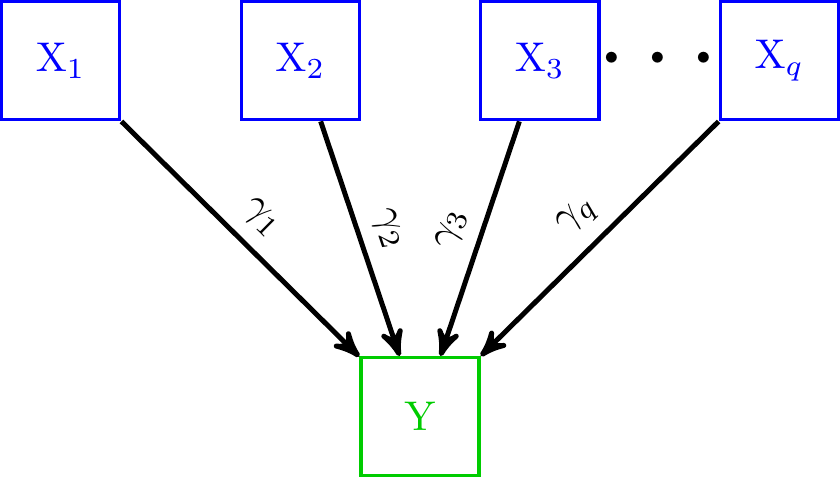
\includegraphics[width=0.8\linewidth]{images/LM1} 

}

\caption{Path Diagram of Linear Model}\label{fig:LM1}
\end{figure}

\begin{example}
A mortgage department of a large bank is studying its recent loans. Of particular interest is how such factors as the value of the home (in thousands of dollars), education level of the head of the household, age of the head of the household and current monthly mortgage payment (in dollars) relate to the family income. Are these variables effect predictors of the income of the household?
\end{example}

\hypertarget{linear-modeling-approach}{%
\section{Linear Modeling Approach}\label{linear-modeling-approach}}

Linear Model (LM) can only measure direct effects
\graffito{Linear Model (LM) can only measure direct effects}

\begin{example}
A mortgage department of a large bank is studying its recent loans. Of particular interest is how such factors as the value of the home (in thousands of dollars), education level of the head of the household, age of the head of the household and current monthly mortgage payment (in dollars) relate to the family income. Are these variables effect predictors of the income of the household?
\end{example}

\begin{figure}[H]

{\centering 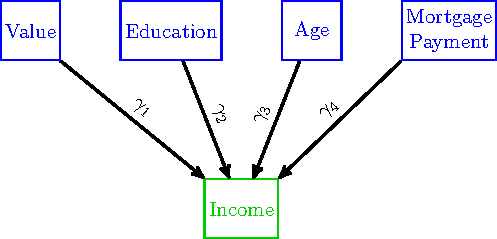
\includegraphics[width=0.8\linewidth]{images/Reg1} 

}

\caption{Path Diagram of Regression}\label{fig:Reg1}
\end{figure}

\begin{Shaded}
\begin{Highlighting}[]
\KeywordTok{load}\NormalTok{(}\StringTok{"Income.RData"}\NormalTok{)}
\CommentTok{# Income}
\KeywordTok{str}\NormalTok{(Income)}
\end{Highlighting}
\end{Shaded}

\begin{verbatim}
'data.frame':   25 obs. of  5 variables:
 $ Income         : num  40.3 39.6 40.8 40.3 40 38.1 40.4 40.7 40.8 37.1 ...
 $ Value          : int  180 121 161 161 179 99 114 202 184 90 ...
 $ Education      : int  14 15 14 14 14 14 15 14 13 14 ...
 $ Age            : int  53 49 44 39 53 46 42 49 37 43 ...
 $ MortgagePayment: int  230 370 397 181 387 304 285 551 370 135 ...
\end{verbatim}

\begin{Shaded}
\begin{Highlighting}[]
\NormalTok{Income.lm.fm1 <-}
\StringTok{  }\KeywordTok{lm}\NormalTok{(}
      \DataTypeTok{formula    =}\NormalTok{ Income }\OperatorTok{~}\StringTok{ }\NormalTok{Value }\OperatorTok{+}\StringTok{ }\NormalTok{Education }\OperatorTok{+}\StringTok{ }\NormalTok{Age }\OperatorTok{+}
\StringTok{                            }\NormalTok{MortgagePayment}
\NormalTok{    , }\DataTypeTok{data       =}\NormalTok{ Income}
  \CommentTok{# , subset}
  \CommentTok{# , weights}
  \CommentTok{# , na.action}
\NormalTok{    , }\DataTypeTok{method      =} \StringTok{"qr"}
\NormalTok{    , }\DataTypeTok{model       =} \OtherTok{TRUE}
\NormalTok{    , }\DataTypeTok{x           =} \OtherTok{FALSE}
\NormalTok{    , }\DataTypeTok{y           =} \OtherTok{FALSE}
\NormalTok{    , }\DataTypeTok{qr          =} \OtherTok{TRUE}
\NormalTok{    , }\DataTypeTok{singular.ok =} \OtherTok{TRUE}
\NormalTok{    , }\DataTypeTok{contrasts   =} \OtherTok{NULL}
  \CommentTok{# , offset}
  \CommentTok{# , ...}
\NormalTok{  )}

\KeywordTok{summary}\NormalTok{(Income.lm.fm1)}
\end{Highlighting}
\end{Shaded}

\begin{verbatim}

Call:
lm(formula = Income ~ Value + Education + Age + MortgagePayment, 
    data = Income, method = "qr", model = TRUE, x = FALSE, y = FALSE, 
    qr = TRUE, singular.ok = TRUE, contrasts = NULL)

Residuals:
     Min       1Q   Median       3Q      Max 
-1.05615 -0.37792 -0.05208  0.47685  1.20372 

Coefficients:
                 Estimate Std. Error t value Pr(>|t|)    
(Intercept)     28.438187   3.442601   8.261 7.08e-08 ***
Value            0.032302   0.005712   5.656 1.55e-05 ***
Education        0.607859   0.277795   2.188   0.0407 *  
Age             -0.037207   0.035780  -1.040   0.3108    
MortgagePayment -0.001345   0.001449  -0.928   0.3644    
---
Signif. codes:  0 '***' 0.001 '**' 0.01 '*' 0.05 '.' 0.1 ' ' 1

Residual standard error: 0.685 on 20 degrees of freedom
Multiple R-squared:  0.6463,    Adjusted R-squared:  0.5756 
F-statistic: 9.137 on 4 and 20 DF,  p-value: 0.0002286
\end{verbatim}

\begin{Shaded}
\begin{Highlighting}[]
\KeywordTok{summary}\NormalTok{(Income.lm.fm1)}\OperatorTok{$}\NormalTok{coef}
\end{Highlighting}
\end{Shaded}

\begin{verbatim}
                    Estimate  Std. Error    t value     Pr(>|t|)
(Intercept)     28.438187019 3.442600555  8.2606700 7.077863e-08
Value            0.032301977 0.005711513  5.6555905 1.553422e-05
Education        0.607858710 0.277794920  2.1881563 4.069801e-02
Age             -0.037207429 0.035780364 -1.0398840 3.108026e-01
MortgagePayment -0.001345319 0.001449331 -0.9282344 3.643539e-01
\end{verbatim}

\begin{figure}[H]

{\centering 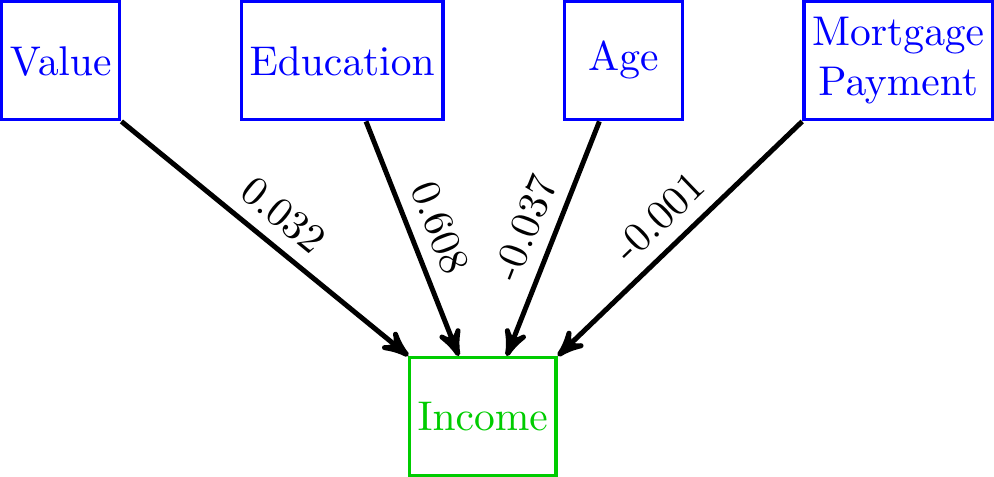
\includegraphics[width=0.8\linewidth]{images/Reg1Values} 

}

\caption{Path Diagram of Regression with estimates of coefficient obtained from \emph{lm}}\label{fig:Reg1Values}
\end{figure}

\hypertarget{strucural-equation-modeling-approach}{%
\section{Strucural Equation Modeling Approach}\label{strucural-equation-modeling-approach}}

Strucural Equation Model (SEM) can measure direct as well as indirect effects

\graffito{Strucural Equation Model (SEM) can measure direct as well as indirect effects}

\begin{example}
A mortgage department of a large bank is studying its recent loans. Of particular interest is how such factors as the value of the home (in thousands of dollars), education level of the head of the household, age of the head of the household and current monthly mortgage payment (in dollars) relate to the family income. Are these variables effect predictors of the income of the household?
\end{example}

\begin{figure}[H]

{\centering 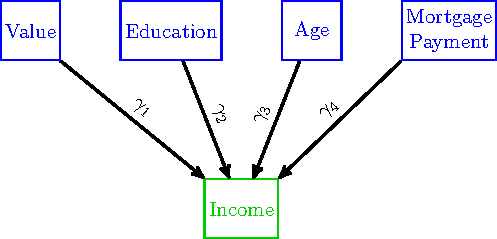
\includegraphics[width=0.8\linewidth]{images/RegSEM1} 

}

\caption{Path Diagram of Regression}\label{fig:RegSEM1}
\end{figure}

\begin{Shaded}
\begin{Highlighting}[]
\KeywordTok{library}\NormalTok{(lavaan)}

\NormalTok{Income.sem.m1 <-}\StringTok{ '}
\StringTok{  # Regressions}
\StringTok{    Income ~ gamma1 * Value + gamma2 * Education +}
\StringTok{             gamma3 * Age   + gamma4 * MortgagePayment}
\StringTok{'}

\NormalTok{Income.sem.fm1 <-}
\StringTok{  }\NormalTok{lavaan}\OperatorTok{::}\KeywordTok{sem}\NormalTok{(}
      \DataTypeTok{model            =}\NormalTok{ Income.sem.m1}
\NormalTok{    , }\DataTypeTok{data             =}\NormalTok{ Income}
\NormalTok{    , }\DataTypeTok{ordered          =} \OtherTok{NULL}
\NormalTok{    , }\DataTypeTok{sampling.weights =} \OtherTok{NULL}
\NormalTok{    , }\DataTypeTok{sample.cov       =} \OtherTok{NULL}
\NormalTok{    , }\DataTypeTok{sample.mean      =} \OtherTok{NULL}
\NormalTok{    , }\DataTypeTok{sample.nobs      =} \OtherTok{NULL}
\NormalTok{    , }\DataTypeTok{group            =} \OtherTok{NULL}
\NormalTok{    , }\DataTypeTok{cluster          =} \OtherTok{NULL}
  \CommentTok{# , constraints      = ""}
\NormalTok{    , }\DataTypeTok{WLS.V            =} \OtherTok{NULL}
\NormalTok{    , }\DataTypeTok{NACOV            =} \OtherTok{NULL}
  \CommentTok{# ,   ...}
\NormalTok{  )}

\CommentTok{# anova(Income.sem.fm1)}
\CommentTok{# coef(Income.sem.fm1)}
\KeywordTok{parameterEstimates}\NormalTok{(Income.sem.fm1, }\DataTypeTok{standardized =} \OtherTok{TRUE}\NormalTok{)}
\end{Highlighting}
\end{Shaded}

\begin{verbatim}
               lhs op             rhs  label       est    se
1           Income  ~           Value gamma1     0.032 0.005
2           Income  ~       Education gamma2     0.608 0.248
3           Income  ~             Age gamma3    -0.037 0.032
4           Income  ~ MortgagePayment gamma4    -0.001 0.001
5           Income ~~          Income            0.375 0.106
6            Value ~~           Value          773.526 0.000
7            Value ~~       Education           -2.619 0.000
8            Value ~~             Age           30.408 0.000
9            Value ~~ MortgagePayment         1087.181 0.000
10       Education ~~       Education            0.458 0.000
11       Education ~~             Age            2.216 0.000
12       Education ~~ MortgagePayment          -14.822 0.000
13             Age ~~             Age           27.840 0.000
14             Age ~~ MortgagePayment          -18.584 0.000
15 MortgagePayment ~~ MortgagePayment        10739.898 0.000
        z pvalue  ci.lower  ci.upper    std.lv std.all   std.nox
1   6.323  0.000     0.022     0.042     0.032   0.872     0.031
2   2.446  0.014     0.121     1.095     0.608   0.399     0.590
3  -1.163  0.245    -0.100     0.026    -0.037  -0.191    -0.036
4  -1.038  0.299    -0.004     0.001    -0.001  -0.135    -0.001
5   3.536  0.000     0.167     0.583     0.375   0.354     0.354
6      NA     NA   773.526   773.526   773.526   1.000   773.526
7      NA     NA    -2.619    -2.619    -2.619  -0.139    -2.619
8      NA     NA    30.408    30.408    30.408   0.207    30.408
9      NA     NA  1087.181  1087.181  1087.181   0.377  1087.181
10     NA     NA     0.458     0.458     0.458   1.000     0.458
11     NA     NA     2.216     2.216     2.216   0.621     2.216
12     NA     NA   -14.822   -14.822   -14.822  -0.211   -14.822
13     NA     NA    27.840    27.840    27.840   1.000    27.840
14     NA     NA   -18.584   -18.584   -18.584  -0.034   -18.584
15     NA     NA 10739.898 10739.898 10739.898   1.000 10739.898
\end{verbatim}

\begin{Shaded}
\begin{Highlighting}[]
\CommentTok{# fitmeasures(Income.sem.fm1)}
\KeywordTok{fitted}\NormalTok{(Income.sem.fm1)}\OperatorTok{$}\NormalTok{cov}
\end{Highlighting}
\end{Shaded}

\begin{verbatim}
                Income    Value     Eductn    Age      
Income              1.061                              
Value              20.800   773.526                    
Education           0.131    -2.619     0.458          
Age                 1.318    30.408     2.216    27.840
MortgagePayment    12.351  1087.181   -14.822   -18.584
                MrtggP   
Income                   
Value                    
Education                
Age                      
MortgagePayment 10739.898
\end{verbatim}

\begin{Shaded}
\begin{Highlighting}[]
\CommentTok{# residuals(Income.sem.fm1, type = "cor")}
\CommentTok{# modificationIndices(Income.sem.fm1)}
\KeywordTok{var}\NormalTok{(Income)}
\end{Highlighting}
\end{Shaded}

\begin{verbatim}
                   Income       Value   Education        Age
Income           1.105433   21.667000   0.1365000   1.373333
Value           21.667000  805.756667  -2.7283333  31.675000
Education        0.136500   -2.728333   0.4766667   2.308333
Age              1.373333   31.675000   2.3083333  29.000000
MortgagePayment 12.865667 1132.480000 -15.4400000 -19.358333
                MortgagePayment
Income                 12.86567
Value                1132.48000
Education             -15.44000
Age                   -19.35833
MortgagePayment     11187.39333
\end{verbatim}

\begin{Shaded}
\begin{Highlighting}[]
\KeywordTok{cor}\NormalTok{(Income)}
\end{Highlighting}
\end{Shaded}

\begin{verbatim}
                   Income      Value  Education         Age
Income          1.0000000  0.7259899  0.1880438  0.24255525
Value           0.7259899  1.0000000 -0.1392157  0.20721237
Education       0.1880438 -0.1392157  1.0000000  0.62085779
Age             0.2425553  0.2072124  0.6208578  1.00000000
MortgagePayment 0.1156915  0.3771934 -0.2114343 -0.03398635
                MortgagePayment
Income               0.11569153
Value                0.37719344
Education           -0.21143430
Age                 -0.03398635
MortgagePayment      1.00000000
\end{verbatim}

\begin{Shaded}
\begin{Highlighting}[]
\CommentTok{# vcov(Income.sem.fm1)}


\KeywordTok{summary}\NormalTok{(}
    \DataTypeTok{object       =}\NormalTok{ Income.sem.fm1}
\NormalTok{  , }\DataTypeTok{header       =} \OtherTok{TRUE}
\NormalTok{  , }\DataTypeTok{fit.measures =} \OtherTok{FALSE}
\NormalTok{  , }\DataTypeTok{estimates    =} \OtherTok{TRUE}
\NormalTok{  , }\DataTypeTok{ci           =} \OtherTok{FALSE}
\NormalTok{  , }\DataTypeTok{fmi          =} \OtherTok{FALSE}
\NormalTok{  , }\DataTypeTok{standardized =} \OtherTok{TRUE}
\NormalTok{  , }\DataTypeTok{rsquare      =} \OtherTok{TRUE}
\NormalTok{  , }\DataTypeTok{std.nox      =} \OtherTok{FALSE}
\NormalTok{  , }\DataTypeTok{modindices   =} \OtherTok{FALSE}
\NormalTok{  , }\DataTypeTok{nd           =}\NormalTok{ 3L}
\NormalTok{)}
\end{Highlighting}
\end{Shaded}

\begin{verbatim}
lavaan 0.6-3 ended normally after 20 iterations

  Optimization method                           NLMINB
  Number of free parameters                          5

  Number of observations                            25

  Estimator                                         ML
  Model Fit Test Statistic                       0.000
  Degrees of freedom                                 0

Parameter Estimates:

  Information                                 Expected
  Information saturated (h1) model          Structured
  Standard Errors                             Standard

Regressions:
                   Estimate   Std.Err  z-value  P(>|z|)
  Income ~                                             
    Value   (gmm1)     0.032    0.005    6.323    0.000
    Educatn (gmm2)     0.608    0.248    2.446    0.014
    Age     (gmm3)    -0.037    0.032   -1.163    0.245
    MrtggPy (gmm4)    -0.001    0.001   -1.038    0.299
   Std.lv   Std.all
                   
     0.032    0.872
     0.608    0.399
    -0.037   -0.191
    -0.001   -0.135

Variances:
                   Estimate   Std.Err  z-value  P(>|z|)
   .Income             0.375    0.106    3.536    0.000
   Std.lv   Std.all
     0.375    0.354

R-Square:
                   Estimate 
    Income             0.646
\end{verbatim}

\begin{figure}[H]

{\centering 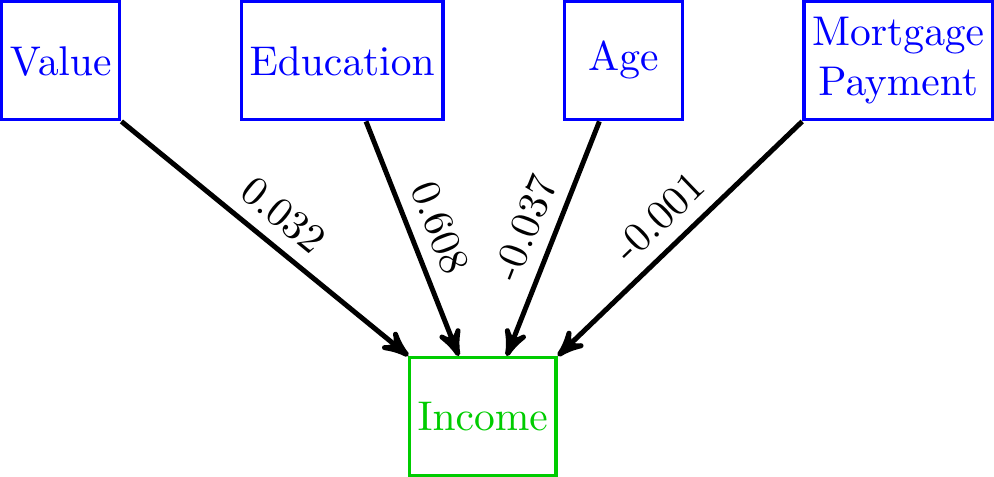
\includegraphics[width=0.8\linewidth]{images/RegSEM1Values} 

}

\caption{Path Diagram of Regression with estimates of coefficient obtained from \emph{sem}}\label{fig:RegSEM1Values}
\end{figure}

\begin{example}
A mortgage department of a large bank is studying its recent loans. Of particular interest is how such factors as the value of the home (in thousands of dollars), education level of the head of the household, age of the head of the household and current monthly mortgage payment (in dollars) relate to the family income. Are these variables effect predictors of the income of the household?
\end{example}

\graffito{Complete path diagram with variances and covariances/correlations}

\begin{figure}[H]

{\centering 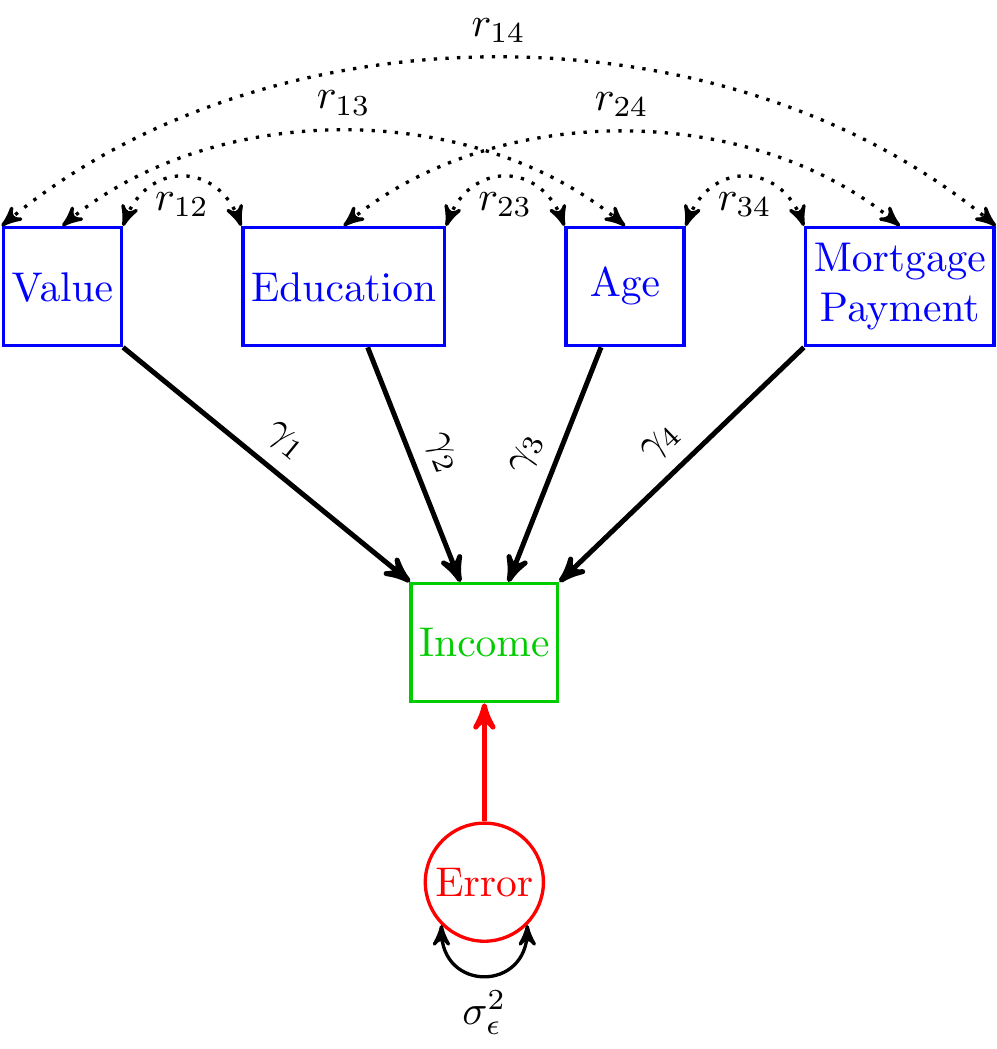
\includegraphics[width=0.8\linewidth]{images/Reg2} 

}

\caption{Path Diagram of Regression}\label{fig:Reg2}
\end{figure}

\begin{Shaded}
\begin{Highlighting}[]
\KeywordTok{library}\NormalTok{(lavaan)}
\NormalTok{Income.sem.m2 <-}\StringTok{ '}
\StringTok{  # Regressions}
\StringTok{    Income ~ gamma1 * Value + gamma2 * Education +}
\StringTok{             gamma3 * Age   + gamma4 * MortgagePayment}

\StringTok{  # Variances and Covariances}
\StringTok{    Value     ~~ r12 * Education}
\StringTok{    Value     ~~ r13 * Age}
\StringTok{    Value     ~~ r14 * MortgagePayment}
\StringTok{    Education ~~ r23 * Age}
\StringTok{    Education ~~ r24 * MortgagePayment}
\StringTok{    Age       ~~ r34 * MortgagePayment}
\StringTok{    Income    ~~ sigma2I * Income}
\StringTok{'}

\NormalTok{Income.sem.fm2 <-}
\StringTok{  }\NormalTok{lavaan}\OperatorTok{::}\KeywordTok{sem}\NormalTok{(}
      \DataTypeTok{model            =}\NormalTok{ Income.sem.m2}
\NormalTok{    , }\DataTypeTok{data             =}\NormalTok{ Income}
\NormalTok{    , }\DataTypeTok{ordered          =} \OtherTok{NULL}
\NormalTok{    , }\DataTypeTok{sampling.weights =} \OtherTok{NULL}
\NormalTok{    , }\DataTypeTok{sample.cov       =} \OtherTok{NULL}
\NormalTok{    , }\DataTypeTok{sample.mean      =} \OtherTok{NULL}
\NormalTok{    , }\DataTypeTok{sample.nobs      =} \OtherTok{NULL}
\NormalTok{    , }\DataTypeTok{group            =} \OtherTok{NULL}
\NormalTok{    , }\DataTypeTok{cluster          =} \OtherTok{NULL}
  \CommentTok{# , constraints      = ""}
\NormalTok{    , }\DataTypeTok{WLS.V            =} \OtherTok{NULL}
\NormalTok{    , }\DataTypeTok{NACOV            =} \OtherTok{NULL}
  \CommentTok{# ,   ...}
\NormalTok{  )}

\CommentTok{# anova(Income.sem.fm2)}
\CommentTok{# coef(Income.sem.fm2)}
\KeywordTok{parameterEstimates}\NormalTok{(Income.sem.fm2, }\DataTypeTok{standardized =} \OtherTok{TRUE}\NormalTok{)}
\end{Highlighting}
\end{Shaded}

\begin{verbatim}
               lhs op             rhs   label       est       se
1           Income  ~           Value  gamma1     0.032    0.005
2           Income  ~       Education  gamma2     0.608    0.248
3           Income  ~             Age  gamma3    -0.037    0.032
4           Income  ~ MortgagePayment  gamma4    -0.001    0.001
5            Value ~~       Education     r12    -2.619    3.799
6            Value ~~             Age     r13    30.408   29.973
7            Value ~~ MortgagePayment     r14  1087.181  616.102
8        Education ~~             Age     r23     2.216    0.840
9        Education ~~ MortgagePayment     r24   -14.822   14.331
10             Age ~~ MortgagePayment     r34   -18.584  109.425
11          Income ~~          Income sigma2I     0.375    0.106
12           Value ~~           Value           773.526  218.786
13       Education ~~       Education             0.458    0.129
14             Age ~~             Age            27.840    7.874
15 MortgagePayment ~~ MortgagePayment         10739.898 3037.702
        z pvalue ci.lower  ci.upper    std.lv std.all std.nox
1   6.323  0.000    0.022     0.042     0.032   0.872   0.872
2   2.446  0.014    0.121     1.095     0.608   0.399   0.399
3  -1.163  0.245   -0.100     0.026    -0.037  -0.191  -0.191
4  -1.038  0.299   -0.004     0.001    -0.001  -0.135  -0.135
5  -0.689  0.491  -10.065     4.827    -2.619  -0.139  -0.139
6   1.015  0.310  -28.338    89.154    30.408   0.207   0.207
7   1.765  0.078 -120.358  2294.719  1087.181   0.377   0.377
8   2.637  0.008    0.569     3.863     2.216   0.621   0.621
9  -1.034  0.301  -42.910    13.265   -14.822  -0.211  -0.211
10 -0.170  0.865 -233.052   195.884   -18.584  -0.034  -0.034
11  3.536  0.000    0.167     0.583     0.375   0.354   0.354
12  3.536  0.000  344.713  1202.340   773.526   1.000   1.000
13  3.536  0.000    0.204     0.711     0.458   1.000   1.000
14  3.536  0.000   12.407    43.273    27.840   1.000   1.000
15  3.536  0.000 4786.112 16693.684 10739.898   1.000   1.000
\end{verbatim}

\begin{Shaded}
\begin{Highlighting}[]
\CommentTok{# fitmeasures(Income.sem.fm2)}
\KeywordTok{fitted}\NormalTok{(Income.sem.fm2)}\OperatorTok{$}\NormalTok{cov}
\end{Highlighting}
\end{Shaded}

\begin{verbatim}
                Income    Value     Eductn    Age      
Income              1.061                              
Value              20.800   773.526                    
Education           0.131    -2.619     0.458          
Age                 1.318    30.408     2.216    27.840
MortgagePayment    12.351  1087.181   -14.822   -18.584
                MrtggP   
Income                   
Value                    
Education                
Age                      
MortgagePayment 10739.898
\end{verbatim}

\begin{Shaded}
\begin{Highlighting}[]
\CommentTok{# residuals(Income.sem.fm2, type = "cor")}
\CommentTok{# modificationIndices(Income.sem.fm2)}
\KeywordTok{var}\NormalTok{(Income)}
\end{Highlighting}
\end{Shaded}

\begin{verbatim}
                   Income       Value   Education        Age
Income           1.105433   21.667000   0.1365000   1.373333
Value           21.667000  805.756667  -2.7283333  31.675000
Education        0.136500   -2.728333   0.4766667   2.308333
Age              1.373333   31.675000   2.3083333  29.000000
MortgagePayment 12.865667 1132.480000 -15.4400000 -19.358333
                MortgagePayment
Income                 12.86567
Value                1132.48000
Education             -15.44000
Age                   -19.35833
MortgagePayment     11187.39333
\end{verbatim}

\begin{Shaded}
\begin{Highlighting}[]
\KeywordTok{cor}\NormalTok{(Income)}
\end{Highlighting}
\end{Shaded}

\begin{verbatim}
                   Income      Value  Education         Age
Income          1.0000000  0.7259899  0.1880438  0.24255525
Value           0.7259899  1.0000000 -0.1392157  0.20721237
Education       0.1880438 -0.1392157  1.0000000  0.62085779
Age             0.2425553  0.2072124  0.6208578  1.00000000
MortgagePayment 0.1156915  0.3771934 -0.2114343 -0.03398635
                MortgagePayment
Income               0.11569153
Value                0.37719344
Education           -0.21143430
Age                 -0.03398635
MortgagePayment      1.00000000
\end{verbatim}

\begin{Shaded}
\begin{Highlighting}[]
\CommentTok{# vcov(Income.sem.fm2)}



\KeywordTok{summary}\NormalTok{(}
    \DataTypeTok{object       =}\NormalTok{ Income.sem.fm2}
\NormalTok{  , }\DataTypeTok{header       =} \OtherTok{TRUE}
\NormalTok{  , }\DataTypeTok{fit.measures =} \OtherTok{TRUE}
\NormalTok{  , }\DataTypeTok{estimates    =} \OtherTok{TRUE}
\NormalTok{  , }\DataTypeTok{ci           =} \OtherTok{FALSE}
\NormalTok{  , }\DataTypeTok{fmi          =} \OtherTok{FALSE}
\NormalTok{  , }\DataTypeTok{standardized =} \OtherTok{TRUE}
\NormalTok{  , }\DataTypeTok{rsquare      =} \OtherTok{TRUE}
\NormalTok{  , }\DataTypeTok{std.nox      =} \OtherTok{FALSE}
\NormalTok{  , }\DataTypeTok{modindices   =} \OtherTok{FALSE}
\NormalTok{  , }\DataTypeTok{nd           =}\NormalTok{ 3L}
\NormalTok{)}
\end{Highlighting}
\end{Shaded}

\begin{verbatim}
lavaan 0.6-3 ended normally after 114 iterations

  Optimization method                           NLMINB
  Number of free parameters                         15

  Number of observations                            25

  Estimator                                         ML
  Model Fit Test Statistic                       0.000
  Degrees of freedom                                 0
  Minimum Function Value               0.0000000000000

Model test baseline model:

  Minimum Function Test Statistic               47.107
  Degrees of freedom                                10
  P-value                                        0.000

User model versus baseline model:

  Comparative Fit Index (CFI)                    1.000
  Tucker-Lewis Index (TLI)                       1.000

Loglikelihood and Information Criteria:

  Loglikelihood user model (H0)               -385.524
  Loglikelihood unrestricted model (H1)       -385.524

  Number of free parameters                         15
  Akaike (AIC)                                 801.048
  Bayesian (BIC)                               819.331
  Sample-size adjusted Bayesian (BIC)          772.815

Root Mean Square Error of Approximation:

  RMSEA                                          0.000
  90 Percent Confidence Interval          0.000  0.000
  P-value RMSEA <= 0.05                             NA

Standardized Root Mean Square Residual:

  SRMR                                           0.000

Parameter Estimates:

  Information                                 Expected
  Information saturated (h1) model          Structured
  Standard Errors                             Standard

Regressions:
                   Estimate   Std.Err  z-value  P(>|z|)
  Income ~                                             
    Value   (gmm1)     0.032    0.005    6.323    0.000
    Educatn (gmm2)     0.608    0.248    2.446    0.014
    Age     (gmm3)    -0.037    0.032   -1.163    0.245
    MrtggPy (gmm4)    -0.001    0.001   -1.038    0.299
   Std.lv   Std.all
                   
     0.032    0.872
     0.608    0.399
    -0.037   -0.191
    -0.001   -0.135

Covariances:
                   Estimate   Std.Err  z-value  P(>|z|)
  Value ~~                                             
    Educatin (r12)    -2.619    3.799   -0.689    0.491
    Age      (r13)    30.408   29.973    1.015    0.310
    MrtggPym (r14)  1087.181  616.102    1.765    0.078
  Education ~~                                         
    Age      (r23)     2.216    0.840    2.637    0.008
    MrtggPym (r24)   -14.822   14.331   -1.034    0.301
  Age ~~                                               
    MrtggPym (r34)   -18.584  109.425   -0.170    0.865
   Std.lv   Std.all
                   
    -2.619   -0.139
    30.408    0.207
  1087.181    0.377
                   
     2.216    0.621
   -14.822   -0.211
                   
   -18.584   -0.034

Variances:
                   Estimate   Std.Err  z-value  P(>|z|)
   .Income  (sg2I)     0.375    0.106    3.536    0.000
    Value            773.526  218.786    3.536    0.000
    Educatn            0.458    0.129    3.536    0.000
    Age               27.840    7.874    3.536    0.000
    MrtggPy        10739.898 3037.702    3.536    0.000
   Std.lv   Std.all
     0.375    0.354
   773.526    1.000
     0.458    1.000
    27.840    1.000
 10739.898    1.000

R-Square:
                   Estimate 
    Income             0.646
\end{verbatim}

\begin{figure}[H]

{\centering 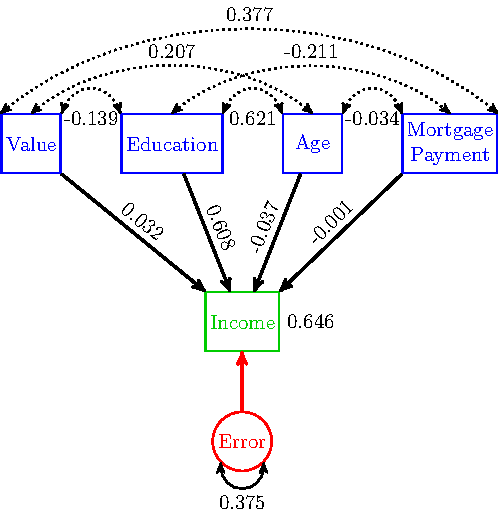
\includegraphics[width=0.8\linewidth]{images/Reg2Values} 

}

\caption{Path Diagram of Regression with estimates of coefficient}\label{fig:Reg2Values}
\end{figure}

\hypertarget{MLM}{%
\chapter{Multivariate Linear Model}\label{MLM}}

\hypertarget{introduction-1}{%
\section{Introduction}\label{introduction-1}}

The model relating the normal dependent variables \(Y_1, Y_2, \cdots, Y_p\) with the explanatory variables \(X_1, X_2, \cdots, X_q\) is

\begin{align*}
Y_{1} & =\gamma_{11}X_{1}+\gamma_{12}X_{2}+\cdots+\gamma_{1q}X_{q}+\epsilon_{1}\\
Y_{2} & =\gamma_{21}X_{1}+\gamma_{22}X_{2}+\cdots+\gamma_{2q}X_{q}+\epsilon_{2}\\
\vdots & \;\qquad\vdots\qquad\qquad\vdots\qquad\;\;\vdots\qquad\;\;\vdots\qquad\;\;\vdots\\
Y_{p} & =\gamma_{p1}X_{1}+\gamma_{p2}X_{2}+\cdots+\gamma_{pq}X_{q}+\epsilon_{p}
\end{align*}

In matrix form the multivariate linear model may be written as

\begin{align}
\begin{bmatrix}Y_{1}\\
Y_{2}\\
\vdots\\
Y_{p}
\end{bmatrix} & =\begin{bmatrix}\gamma_{11} & \gamma_{12} & \ldots & \gamma_{1q}\\
\gamma_{21} & \gamma_{22} & \ldots & \gamma_{2q}\\
\vdots & \vdots & \ddots & \vdots\\
\gamma_{p1} & \gamma_{p2} & \ldots & \gamma_{pq}
\end{bmatrix}\begin{bmatrix}X_{1}\\
X_{2}\\
\vdots\\
X_{q}
\end{bmatrix}+\begin{bmatrix}\epsilon_{1}\\
\epsilon_{2}\\
\vdots\\
\epsilon_{p}
\end{bmatrix}\label{eq:MLM1}\\
\mathbf{y} & =\bm{\Gamma}\mathbf{x}+\bm{\epsilon}\label{eq:MLM2}
\end{align}

Therefore, the multivariate linear model for the \(i\)-th observation is

\begin{equation}
\mathbf{y}_{i}  = \bm{\Gamma}\bm{x}_{i} +  \bm{\epsilon}_{i}
\label{eq:MLM3}
\end{equation}

The \(\mathbf{y}_{i}\) \(\left(p\times1\right)\) and the \(\mathbf{x}_{i}\)
\(\left(q\times1\right)\) vectors are observed variables, \(\bm{\Gamma}\) (Gamma) is the \(p\times q\) coefficient matrix for the effects of \(\mathbf{x}_{i}\) on \(\mathbf{y}_{i}\). \(\bm{\epsilon}_{i}\) (epsilon) is the disturbance vector that is assumed to have an expected value of zero \(\left[\mathbb{E}\left(\bm{\epsilon}_{i}\right)=\mathbf{0}\right]\).

\begin{figure}[H]

{\centering 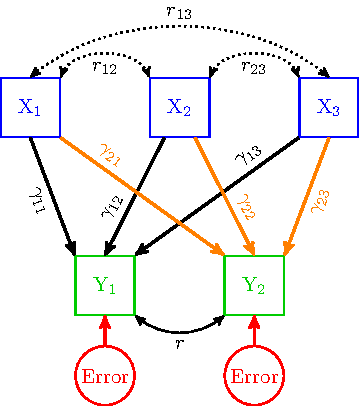
\includegraphics[width=0.8\linewidth]{images/MLM1} 

}

\caption{Path Diagram for Multivariate Linear Model}\label{fig:MLM1}
\end{figure}

\hypertarget{SEMO}{%
\chapter{Structural Equation Modeling with Observed Variables}\label{SEMO}}

\hypertarget{introduction-2}{%
\section{Introduction}\label{introduction-2}}

The general model of structural equations with observed variables is

\scriptsize

\begin{align*}
Y_{1} & =\beta_{12}Y_{2}+\beta_{13}Y_{3}+\cdots+\beta_{1p}Y_{p}\qquad\quad+\gamma_{11}X_{1}+\gamma_{12}X_{2}+\cdots+\gamma_{1q}X_{q}+\epsilon_{1}\\
Y_{2} & =\beta_{21}Y_{1}+\beta_{23}Y_{3}+\cdots+\beta_{2p}Y_{p}\qquad\quad+\gamma_{21}X_{1}+\gamma_{22}X_{2}+\cdots+\gamma_{2q}X_{q}+\epsilon_{2}\\
\vdots & \;\qquad\vdots\qquad\quad\;\;\vdots\qquad\quad\vdots\qquad\;\;\vdots\qquad\qquad\quad\vdots\qquad\quad\;\;\vdots\qquad\quad\;\;\;\vdots\qquad\vdots\qquad\quad\;\;\;\vdots\\
Y_{p} & =\beta_{p1}Y_{1}+\beta_{p2}Y_{2}+\cdots+\beta_{p\left(p-1\right)}Y_{p-1}+\gamma_{p1}X_{1}+\gamma_{p2}X_{2}+\cdots+\gamma_{pq}X_{q}+\epsilon_{p}
\end{align*}

\normalsize

In matrix form the general model of structural equations with observed variables may be written as

\scriptsize

\begin{align}
\begin{bmatrix}Y_{1}\\
Y_{2}\\
\vdots\\
Y_{p}
\end{bmatrix} & =\begin{bmatrix}0 & \beta_{12} & \ldots & \beta_{1p}\\
\beta_{21} & 0 & \ldots & \beta_{2p}\\
\vdots & \vdots & \ddots & \vdots\\
\beta_{p1} & \beta_{p2} & \ldots & 0
\end{bmatrix}\begin{bmatrix}Y_{1}\\
Y_{2}\\
\vdots\\
Y_{p}
\end{bmatrix}+\begin{bmatrix}\gamma_{11} & \gamma_{12} & \ldots & \gamma_{1q}\\
\gamma_{21} & \gamma_{22} & \ldots & \gamma_{2q}\\
\vdots & \vdots & \ddots & \vdots\\
\gamma_{p1} & \gamma_{p2} & \ldots & \gamma_{pq}
\end{bmatrix}\begin{bmatrix}X_{1}\\
X_{2}\\
\vdots\\
X_{q}
\end{bmatrix}+\begin{bmatrix}\epsilon_{1}\\
\epsilon_{2}\\
\vdots\\
\epsilon_{p}
\end{bmatrix}\label{eq:SEMO1}\\
\mathbf{y} & =\mathbf{B}\mathbf{y}+\bm{\Gamma}\mathbf{x}+\bm{\epsilon}\label{eq:SEMO2}
\end{align}

\normalsize

Therefore, the general model of structural equations with observed variables for the \(i\)-th observation is

\begin{equation}
\mathbf{y}_{i}  =\mathbf{B} \mathbf{y}_{i} + \bm{\Gamma}\bm{x}_{i} +  \bm{\epsilon}_{i}
\label{eq:SEMO3}
\end{equation}

The \(\mathbf{y}_{i}\) \(\left(p\times1\right)\) and the \(\mathbf{x}_{i}\)
\(\left(q\times1\right)\) vectors are observed variables, \(\mathbf{B}\)
is the \(p\times p\) coefficient matrix showing the influence of the endogenous variables on each other; \(\bm{\Gamma}\) (Gamma)
is the \(p\times q\) coefficient matrix for the effects of \(\mathbf{x}_{i}\)
on \(\mathbf{y}_{i}\). The matrix \(\left(\mathbf{I}-\mathbf{B}\right)\)
is non-singular. \(\bm{\epsilon}_{i}\) (zeta) is the disturbance vector
that is assumed to have an expected value of zero \(\left[\mathbb{E}\left(\bm{\epsilon}_{i}\right)=\mathbf{0}\right]\).

\begin{figure}[H]

{\centering 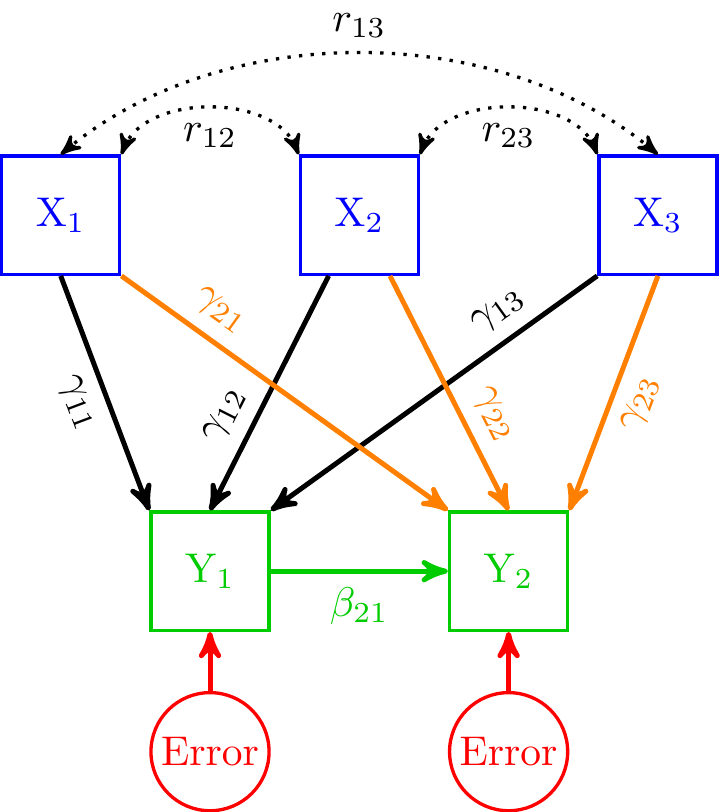
\includegraphics[width=0.8\linewidth]{images/SEMO1} 

}

\caption{Path Diagram for Structural Equations Model with Observed Variables}\label{fig:SEMO1}
\end{figure}

\graffito{Complete path diagram with direct as well as indirect effects and corresponding variances and covariances/correlations}

\begin{example}
A mortgage department of a large bank is studying its recent loans. Of particular interest is how such factors as the value of the home (in thousands of dollars), education level of the head of the household, age of the head of the household and current monthly mortgage payment (in dollars) relate to the family income. Are these variables effect predictors of the income of the household?
\end{example}

\begin{figure}[H]

{\centering 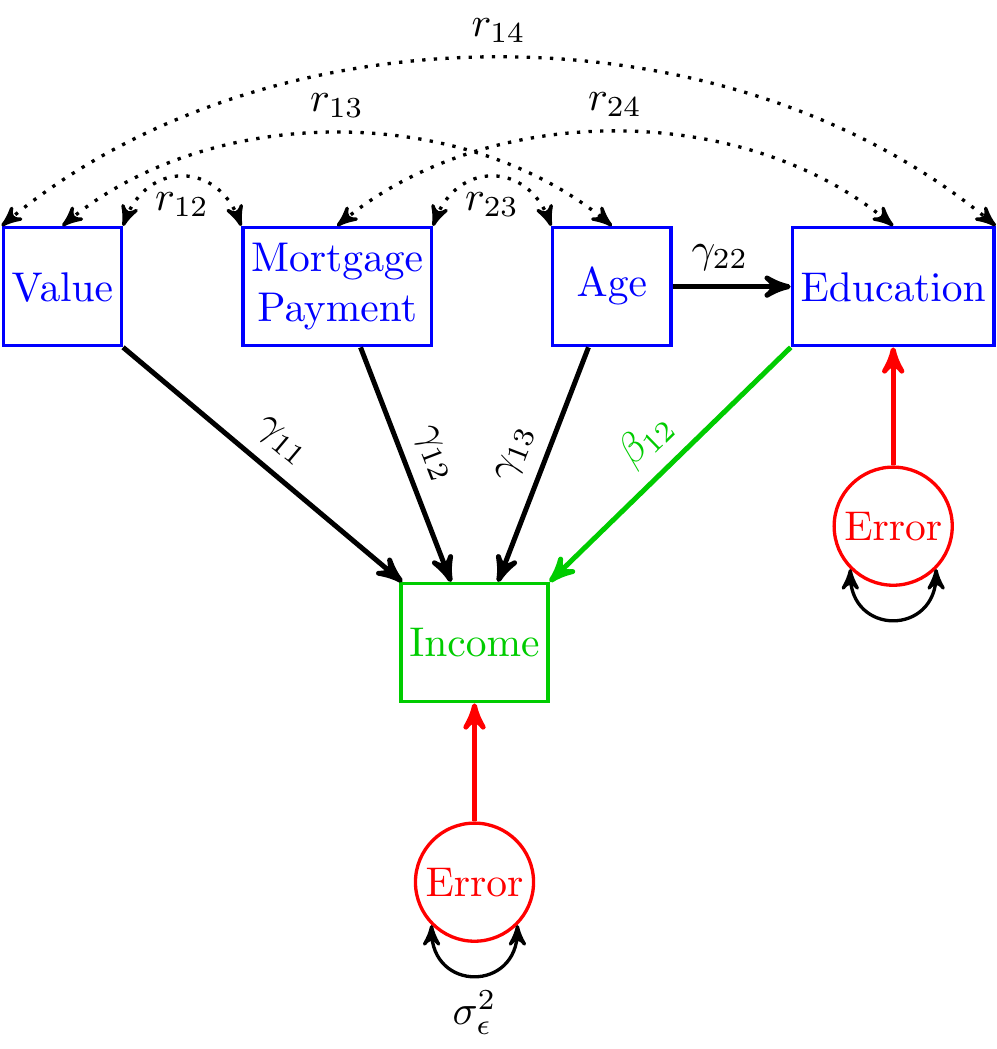
\includegraphics[width=0.8\linewidth]{images/Reg3} 

}

\caption{Path Diagram with Indirecet Effects}\label{fig:Reg3}
\end{figure}

\begin{Shaded}
\begin{Highlighting}[]
\KeywordTok{load}\NormalTok{(}\StringTok{"Income.RData"}\NormalTok{)}
\CommentTok{# Income}
\KeywordTok{str}\NormalTok{(Income)}
\end{Highlighting}
\end{Shaded}

\begin{verbatim}
'data.frame':   25 obs. of  5 variables:
 $ Income         : num  40.3 39.6 40.8 40.3 40 38.1 40.4 40.7 40.8 37.1 ...
 $ Value          : int  180 121 161 161 179 99 114 202 184 90 ...
 $ Education      : int  14 15 14 14 14 14 15 14 13 14 ...
 $ Age            : int  53 49 44 39 53 46 42 49 37 43 ...
 $ MortgagePayment: int  230 370 397 181 387 304 285 551 370 135 ...
\end{verbatim}

\begin{Shaded}
\begin{Highlighting}[]
\KeywordTok{library}\NormalTok{(lavaan)}

\NormalTok{Income.sem.m3 <-}\StringTok{ '}
\StringTok{  # Regressions}
\StringTok{    Income    ~ beta12 * Education + gamma11 * Value +}
\StringTok{                gamma12 * MortgagePayment + gamma13 * Age}
\StringTok{    Education ~ gamma22 * Age}

\StringTok{  # Variances and Covariances}
\StringTok{    Value           ~~ r12 * MortgagePayment}
\StringTok{    Value           ~~ r13 * Age}
\StringTok{    Value           ~~ r14 * Education}
\StringTok{    MortgagePayment ~~ r23 * Age}
\StringTok{    MortgagePayment ~~ r24 *Education}
\StringTok{    Education       ~~ sigma2E * Education}
\StringTok{    Income          ~~ sigma2I * Income}

\StringTok{# Indirect Effects}
\StringTok{  IndEf := gamma22*beta12}

\StringTok{# Total Effects (Direct + Indirect Effets)}
\StringTok{  TotEf := gamma13 + (gamma22*beta12)}
\StringTok{'}

\NormalTok{Income.sem.fm3 <-}
\StringTok{  }\NormalTok{lavaan}\OperatorTok{::}\KeywordTok{sem}\NormalTok{(}
      \DataTypeTok{model            =}\NormalTok{ Income.sem.m3}
\NormalTok{    , }\DataTypeTok{data             =}\NormalTok{ Income}
\NormalTok{    , }\DataTypeTok{ordered          =} \OtherTok{NULL}
\NormalTok{    , }\DataTypeTok{sampling.weights =} \OtherTok{NULL}
\NormalTok{    , }\DataTypeTok{sample.cov       =} \OtherTok{NULL}
\NormalTok{    , }\DataTypeTok{sample.mean      =} \OtherTok{NULL}
\NormalTok{    , }\DataTypeTok{sample.nobs      =} \OtherTok{NULL}
\NormalTok{    , }\DataTypeTok{group            =} \OtherTok{NULL}
\NormalTok{    , }\DataTypeTok{cluster          =} \OtherTok{NULL}
  \CommentTok{# , constraints      = ""}
\NormalTok{    , }\DataTypeTok{WLS.V            =} \OtherTok{NULL}
\NormalTok{    , }\DataTypeTok{NACOV            =} \OtherTok{NULL}
  \CommentTok{# ,   ...}
\NormalTok{  )}

\CommentTok{# anova(Income.sem.fm3)}
\CommentTok{# coef(Income.sem.fm3)}
\KeywordTok{parameterEstimates}\NormalTok{(Income.sem.fm3, }\DataTypeTok{standardized =} \OtherTok{TRUE}\NormalTok{)}
\end{Highlighting}
\end{Shaded}

\begin{verbatim}
               lhs op                      rhs   label       est
1           Income  ~                Education  beta12     0.608
2           Income  ~                    Value gamma11     0.032
3           Income  ~          MortgagePayment gamma12    -0.001
4           Income  ~                      Age gamma13    -0.037
5        Education  ~                      Age gamma22     0.080
6            Value ~~          MortgagePayment     r12  1087.181
7            Value ~~                      Age     r13    30.408
8        Education ~~                    Value     r14    -5.040
9  MortgagePayment ~~                      Age     r23   -18.584
10       Education ~~          MortgagePayment     r24   -13.343
11       Education ~~                Education sigma2E     0.281
12          Income ~~                   Income sigma2I     0.375
13           Value ~~                    Value           773.526
14 MortgagePayment ~~          MortgagePayment         10739.898
15             Age ~~                      Age            27.840
16           IndEf :=           gamma22*beta12   IndEf     0.048
17           TotEf := gamma13+(gamma22*beta12)   TotEf     0.011
         se      z pvalue ci.lower  ci.upper    std.lv std.all
1     0.248  2.446  0.014    0.121     1.095     0.608   0.399
2     0.005  6.323  0.000    0.022     0.042     0.032   0.872
3     0.001 -1.038  0.299   -0.004     0.001    -0.001  -0.135
4     0.032 -1.163  0.245   -0.100     0.026    -0.037  -0.191
5     0.020  3.960  0.000    0.040     0.119     0.080   0.621
6   616.102  1.765  0.078 -120.358  2294.719  1087.181   0.377
7    29.973  1.015  0.310  -28.338    89.154    30.408   0.207
8     3.057 -1.649  0.099  -11.031     0.951    -5.040  -0.342
9   109.425 -0.170  0.865 -233.052   195.884   -18.584  -0.034
10   11.304 -1.180  0.238  -35.499     8.813   -13.343  -0.243
11    0.080  3.536  0.000    0.125     0.437     0.281   0.615
12    0.106  3.536  0.000    0.167     0.583     0.375   0.354
13  218.786  3.536  0.000  344.713  1202.340   773.526   1.000
14 3037.702  3.536  0.000 4786.111 16693.684 10739.898   1.000
15    7.874  3.536  0.000   12.407    43.273    27.840   1.000
16    0.023  2.081  0.037    0.003     0.094     0.048   0.248
17    0.027  0.415  0.678   -0.042     0.064     0.011   0.057
   std.nox
1    0.399
2    0.872
3   -0.135
4   -0.191
5    0.621
6    0.377
7    0.207
8   -0.342
9   -0.034
10  -0.243
11   0.615
12   0.354
13   1.000
14   1.000
15   1.000
16   0.248
17   0.057
\end{verbatim}

\begin{Shaded}
\begin{Highlighting}[]
\CommentTok{# fitmeasures(Income.sem.fm3)}
\KeywordTok{fitted}\NormalTok{(Income.sem.fm3)}\OperatorTok{$}\NormalTok{cov}
\end{Highlighting}
\end{Shaded}

\begin{verbatim}
                Income    Eductn    Value     MrtggP   
Income              1.061                              
Education           0.131     0.458                    
Value              20.800    -2.619   773.526          
MortgagePayment    12.351   -14.822  1087.181 10739.898
Age                 1.318     2.216    30.408   -18.584
                Age      
Income                   
Education                
Value                    
MortgagePayment          
Age                27.840
\end{verbatim}

\begin{Shaded}
\begin{Highlighting}[]
\CommentTok{# residuals(Income.sem.fm3, type = "cor")}
\CommentTok{# modificationIndices(Income.sem.fm3)}
\KeywordTok{var}\NormalTok{(Income)}
\end{Highlighting}
\end{Shaded}

\begin{verbatim}
                   Income       Value   Education        Age
Income           1.105433   21.667000   0.1365000   1.373333
Value           21.667000  805.756667  -2.7283333  31.675000
Education        0.136500   -2.728333   0.4766667   2.308333
Age              1.373333   31.675000   2.3083333  29.000000
MortgagePayment 12.865667 1132.480000 -15.4400000 -19.358333
                MortgagePayment
Income                 12.86567
Value                1132.48000
Education             -15.44000
Age                   -19.35833
MortgagePayment     11187.39333
\end{verbatim}

\begin{Shaded}
\begin{Highlighting}[]
\CommentTok{# vcov(Income.sem.fm3)}


\KeywordTok{summary}\NormalTok{(}
    \DataTypeTok{object       =}\NormalTok{ Income.sem.fm3}
\NormalTok{  , }\DataTypeTok{header       =} \OtherTok{TRUE}
\NormalTok{  , }\DataTypeTok{fit.measures =} \OtherTok{FALSE}
\NormalTok{  , }\DataTypeTok{estimates    =} \OtherTok{TRUE}
\NormalTok{  , }\DataTypeTok{ci           =} \OtherTok{FALSE}
\NormalTok{  , }\DataTypeTok{fmi          =} \OtherTok{FALSE}
\NormalTok{  , }\DataTypeTok{standardized =} \OtherTok{TRUE}
\NormalTok{  , }\DataTypeTok{rsquare      =} \OtherTok{TRUE}
\NormalTok{  , }\DataTypeTok{std.nox      =} \OtherTok{FALSE}
\NormalTok{  , }\DataTypeTok{modindices   =} \OtherTok{FALSE}
\NormalTok{  , }\DataTypeTok{nd           =}\NormalTok{ 3L}
\NormalTok{)}
\end{Highlighting}
\end{Shaded}

\begin{verbatim}
lavaan 0.6-3 ended normally after 112 iterations

  Optimization method                           NLMINB
  Number of free parameters                         15

  Number of observations                            25

  Estimator                                         ML
  Model Fit Test Statistic                       0.000
  Degrees of freedom                                 0
  Minimum Function Value               0.0000000000000

Parameter Estimates:

  Information                                 Expected
  Information saturated (h1) model          Structured
  Standard Errors                             Standard

Regressions:
                   Estimate   Std.Err  z-value  P(>|z|)
  Income ~                                             
    Educatn (bt12)     0.608    0.248    2.446    0.014
    Value   (gm11)     0.032    0.005    6.323    0.000
    MrtggPy (gm12)    -0.001    0.001   -1.038    0.299
    Age     (gm13)    -0.037    0.032   -1.163    0.245
  Education ~                                          
    Age     (gm22)     0.080    0.020    3.960    0.000
   Std.lv   Std.all
                   
     0.608    0.399
     0.032    0.872
    -0.001   -0.135
    -0.037   -0.191
                   
     0.080    0.621

Covariances:
                     Estimate   Std.Err  z-value  P(>|z|)
  Value ~~                                               
    MrtggPym (r12)    1087.181  616.102    1.765    0.078
    Age      (r13)      30.408   29.973    1.015    0.310
 .Education ~~                                           
    Value    (r14)      -5.040    3.057   -1.649    0.099
  MortgagePayment ~~                                     
    Age      (r23)     -18.584  109.425   -0.170    0.865
 .Education ~~                                           
    MrtggPym (r24)     -13.343   11.304   -1.180    0.238
   Std.lv   Std.all
                   
  1087.181    0.377
    30.408    0.207
                   
    -5.040   -0.342
                   
   -18.584   -0.034
                   
   -13.343   -0.243

Variances:
                   Estimate   Std.Err  z-value  P(>|z|)
   .Educatn (sg2E)     0.281    0.080    3.536    0.000
   .Income  (sg2I)     0.375    0.106    3.536    0.000
    Value            773.526  218.786    3.536    0.000
    MrtggPy        10739.898 3037.702    3.536    0.000
    Age               27.840    7.874    3.536    0.000
   Std.lv   Std.all
     0.281    0.615
     0.375    0.354
   773.526    1.000
 10739.898    1.000
    27.840    1.000

R-Square:
                   Estimate 
    Education          0.385
    Income             0.646

Defined Parameters:
                   Estimate   Std.Err  z-value  P(>|z|)
    IndEf              0.048    0.023    2.081    0.037
    TotEf              0.011    0.027    0.415    0.678
   Std.lv   Std.all
     0.048    0.248
     0.011    0.057
\end{verbatim}

\begin{figure}[H]

{\centering 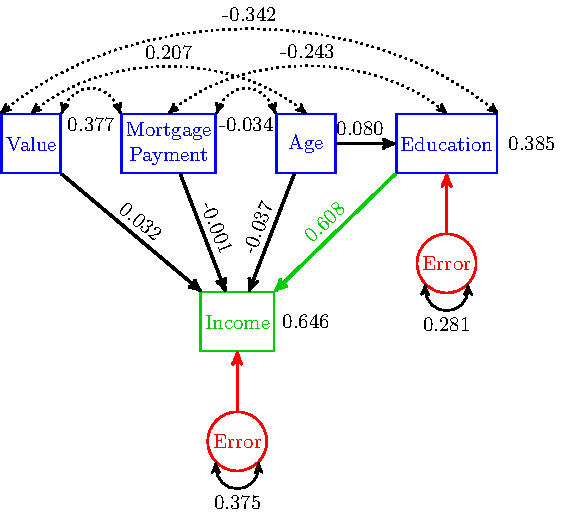
\includegraphics[width=0.8\linewidth]{images/Reg3Values} 

}

\caption{Path Diagram with estimates of coefficient including Indirecet Effects}\label{fig:Reg3Values}
\end{figure}

\begin{example}
Job Performance of Farm Managers

\begin{tabular}{lclp{7cm}}
Knowledge  & : & (26 Items) & \tabularnewline
Value & : & (30 Items) & Tendency to rationally evaluate means to an economic end\tabularnewline
Satisfaction & : & (11 Items) & Gratification from the managerial role\tabularnewline
Performance & : & (24 Items) & \tabularnewline
\end{tabular}


\end{example}

\begin{figure}[H]

{\centering 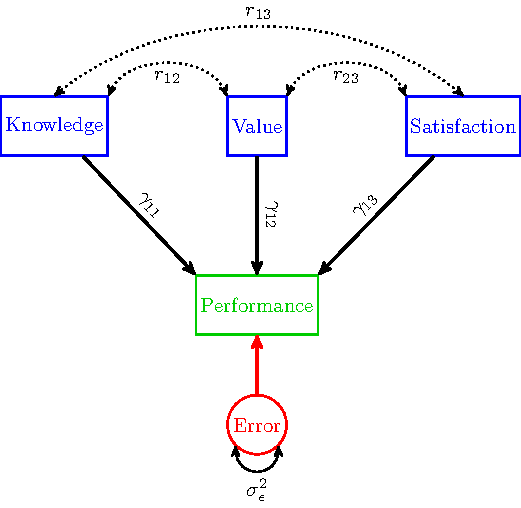
\includegraphics[width=0.8\linewidth]{images/Warren5V1} 

}

\caption{Path Diagram for job performance of farm managers}\label{fig:Warren5V1}
\end{figure}

\begin{Shaded}
\begin{Highlighting}[]
\KeywordTok{library}\NormalTok{(lavaan)}

\NormalTok{Warren5V <-}
\StringTok{  }\KeywordTok{matrix}\NormalTok{(}
    \DataTypeTok{data =}
      \KeywordTok{c}\NormalTok{(}
        \FloatTok{0.0209}\NormalTok{, }\FloatTok{0.0177}\NormalTok{,  }\FloatTok{0.0245}\NormalTok{,     }\FloatTok{0.0046}\NormalTok{,}
        \FloatTok{0.0177}\NormalTok{, }\FloatTok{0.0520}\NormalTok{,  }\FloatTok{0.0280}\NormalTok{,     }\FloatTok{0.0044}\NormalTok{,}
        \FloatTok{0.0245}\NormalTok{, }\FloatTok{0.0280}\NormalTok{,  }\FloatTok{0.1212}\NormalTok{,    }\FloatTok{-0.0063}\NormalTok{,}
        \FloatTok{0.0046}\NormalTok{, }\FloatTok{0.0044}\NormalTok{, }\FloatTok{-0.0063}\NormalTok{,     }\FloatTok{0.0901}
\NormalTok{      )}
\NormalTok{    , }\DataTypeTok{nrow  =} \DecValTok{4}
\NormalTok{    , }\DataTypeTok{ncol  =} \DecValTok{4}
\NormalTok{    , }\DataTypeTok{byrow =} \OtherTok{TRUE}
\NormalTok{    , }\DataTypeTok{dimnames =} \KeywordTok{list}\NormalTok{(}\KeywordTok{c}\NormalTok{(}\StringTok{"Performance"}\NormalTok{,  }\StringTok{"Knowledge"}\NormalTok{,}
                        \StringTok{"Value"}\NormalTok{,    }\StringTok{"Satisfaction"}\NormalTok{)}
\NormalTok{                      , }\KeywordTok{c}\NormalTok{(}\StringTok{"Performance"}\NormalTok{,    }\StringTok{"Knowledge"}\NormalTok{,}
                          \StringTok{"Value"}\NormalTok{,  }\StringTok{"Satisfaction"}\NormalTok{))}
\NormalTok{    )}

\NormalTok{Warren5V}
\end{Highlighting}
\end{Shaded}

\begin{verbatim}
             Performance Knowledge   Value Satisfaction
Performance       0.0209    0.0177  0.0245       0.0046
Knowledge         0.0177    0.0520  0.0280       0.0044
Value             0.0245    0.0280  0.1212      -0.0063
Satisfaction      0.0046    0.0044 -0.0063       0.0901
\end{verbatim}

\begin{Shaded}
\begin{Highlighting}[]
\NormalTok{Warren5V.sem.m1 <-}\StringTok{ '}
\StringTok{  # Regressions}
\StringTok{    Performance ~ gamma11 * Knowledge + gamma12 * Value +}
\StringTok{                  gamma13 * Satisfaction}

\StringTok{  # Variances and Covariances}
\StringTok{    Knowledge   ~~ r12 * Value}
\StringTok{    Knowledge   ~~ r13 * Satisfaction}
\StringTok{    Value       ~~ r23 * Satisfaction}
\StringTok{    Performance ~~ sigma2P * Performance}
\StringTok{'}

\NormalTok{Warren5V.sem.fm1 <-}
\StringTok{  }\NormalTok{lavaan}\OperatorTok{::}\KeywordTok{sem}\NormalTok{(}
      \DataTypeTok{model            =}\NormalTok{ Warren5V.sem.m1}
  \CommentTok{# , data}
\NormalTok{    , }\DataTypeTok{ordered          =} \OtherTok{NULL}
\NormalTok{    , }\DataTypeTok{sampling.weights =} \OtherTok{NULL}
\NormalTok{    , }\DataTypeTok{sample.cov       =}\NormalTok{ Warren5V}
\NormalTok{    , }\DataTypeTok{sample.mean      =} \OtherTok{NULL}
\NormalTok{    , }\DataTypeTok{sample.nobs      =} \DecValTok{98}
\NormalTok{    , }\DataTypeTok{group            =} \OtherTok{NULL}
\NormalTok{    , }\DataTypeTok{cluster          =} \OtherTok{NULL}
  \CommentTok{# , constraints      = ""}
\NormalTok{    , }\DataTypeTok{WLS.V            =} \OtherTok{NULL}
\NormalTok{    , }\DataTypeTok{NACOV            =} \OtherTok{NULL}
  \CommentTok{# ,   ...}
\NormalTok{  )}

\CommentTok{# methods(class = class(Warren5V.sem.fm1))}
\CommentTok{# anova(Warren5V.sem.fm1)}
\CommentTok{# coef(Warren5V.sem.fm1)}
\KeywordTok{parameterEstimates}\NormalTok{(Warren5V.sem.fm1, }\DataTypeTok{standardized =} \OtherTok{TRUE}\NormalTok{)}
\end{Highlighting}
\end{Shaded}

\begin{verbatim}
            lhs op          rhs   label    est    se      z
1   Performance  ~    Knowledge gamma11  0.258 0.053  4.847
2   Performance  ~        Value gamma12  0.145 0.035  4.158
3   Performance  ~ Satisfaction gamma13  0.049 0.038  1.281
4     Knowledge ~~        Value     r12  0.028 0.008  3.293
5     Knowledge ~~ Satisfaction     r13  0.004 0.007  0.635
6         Value ~~ Satisfaction     r23 -0.006 0.010 -0.596
7   Performance ~~  Performance sigma2P  0.012 0.002  7.000
8     Knowledge ~~    Knowledge          0.051 0.007  7.000
9         Value ~~        Value          0.120 0.017  7.000
10 Satisfaction ~~ Satisfaction          0.089 0.013  7.000
   pvalue ci.lower ci.upper std.lv std.all std.nox
1   0.000    0.154    0.363  0.258   0.407   0.407
2   0.000    0.077    0.213  0.145   0.349   0.349
3   0.200   -0.026    0.123  0.049   0.101   0.101
4   0.001    0.011    0.044  0.028   0.353   0.353
5   0.525   -0.009    0.018  0.004   0.064   0.064
6   0.551   -0.027    0.014 -0.006  -0.060  -0.060
7   0.000    0.009    0.016  0.012   0.601   0.601
8   0.000    0.037    0.066  0.051   1.000   1.000
9   0.000    0.086    0.154  0.120   1.000   1.000
10  0.000    0.064    0.114  0.089   1.000   1.000
\end{verbatim}

\begin{Shaded}
\begin{Highlighting}[]
\CommentTok{# fitmeasures(Warren5V.sem.fm1)}
\KeywordTok{fitted}\NormalTok{(Warren5V.sem.fm1)}\OperatorTok{$}\NormalTok{cov}
\end{Highlighting}
\end{Shaded}

\begin{verbatim}
             Prfrmn Knwldg Value  Stsfct
Performance   0.021                     
Knowledge     0.018  0.051              
Value         0.024  0.028  0.120       
Satisfaction  0.005  0.004 -0.006  0.089
\end{verbatim}

\begin{Shaded}
\begin{Highlighting}[]
\CommentTok{# residuals(Warren5V.sem.fm1, type = "cor")}
\CommentTok{# modificationIndices(Warren5V.sem.fm1)}
\NormalTok{Warren5V}
\end{Highlighting}
\end{Shaded}

\begin{verbatim}
             Performance Knowledge   Value Satisfaction
Performance       0.0209    0.0177  0.0245       0.0046
Knowledge         0.0177    0.0520  0.0280       0.0044
Value             0.0245    0.0280  0.1212      -0.0063
Satisfaction      0.0046    0.0044 -0.0063       0.0901
\end{verbatim}

\begin{Shaded}
\begin{Highlighting}[]
\CommentTok{# vcov(Warren5V.sem.fm1)}


\KeywordTok{summary}\NormalTok{(}
    \DataTypeTok{object       =}\NormalTok{ Warren5V.sem.fm1}
\NormalTok{  , }\DataTypeTok{header       =} \OtherTok{TRUE}
\NormalTok{  , }\DataTypeTok{fit.measures =} \OtherTok{FALSE}
\NormalTok{  , }\DataTypeTok{estimates    =} \OtherTok{TRUE}
\NormalTok{  , }\DataTypeTok{ci           =} \OtherTok{FALSE}
\NormalTok{  , }\DataTypeTok{fmi          =} \OtherTok{FALSE}
\NormalTok{  , }\DataTypeTok{standardized =} \OtherTok{TRUE}
\NormalTok{  , }\DataTypeTok{rsquare      =} \OtherTok{TRUE}
\NormalTok{  , }\DataTypeTok{std.nox      =} \OtherTok{FALSE}
\NormalTok{  , }\DataTypeTok{modindices   =} \OtherTok{FALSE}
\NormalTok{  , }\DataTypeTok{nd           =}\NormalTok{ 3L}
\NormalTok{)}
\end{Highlighting}
\end{Shaded}

\begin{verbatim}
lavaan 0.6-3 ended normally after 46 iterations

  Optimization method                           NLMINB
  Number of free parameters                         10

  Number of observations                            98

  Estimator                                         ML
  Model Fit Test Statistic                       0.000
  Degrees of freedom                                 0

Parameter Estimates:

  Information                                 Expected
  Information saturated (h1) model          Structured
  Standard Errors                             Standard

Regressions:
                   Estimate  Std.Err  z-value  P(>|z|)   Std.lv
  Performance ~                                                
    Knowldg (gm11)    0.258    0.053    4.847    0.000    0.258
    Value   (gm12)    0.145    0.035    4.158    0.000    0.145
    Stsfctn (gm13)    0.049    0.038    1.281    0.200    0.049
  Std.all
         
    0.407
    0.349
    0.101

Covariances:
                   Estimate  Std.Err  z-value  P(>|z|)   Std.lv
  Knowledge ~~                                                 
    Value    (r12)    0.028    0.008    3.293    0.001    0.028
    Satsfctn (r13)    0.004    0.007    0.635    0.525    0.004
  Value ~~                                                     
    Satsfctn (r23)   -0.006    0.010   -0.596    0.551   -0.006
  Std.all
         
    0.353
    0.064
         
   -0.060

Variances:
                   Estimate  Std.Err  z-value  P(>|z|)   Std.lv
   .Prfrmnc (sg2P)    0.012    0.002    7.000    0.000    0.012
    Knowldg           0.051    0.007    7.000    0.000    0.051
    Value             0.120    0.017    7.000    0.000    0.120
    Stsfctn           0.089    0.013    7.000    0.000    0.089
  Std.all
    0.601
    1.000
    1.000
    1.000

R-Square:
                   Estimate
    Performance       0.399
\end{verbatim}

\begin{figure}[H]

{\centering 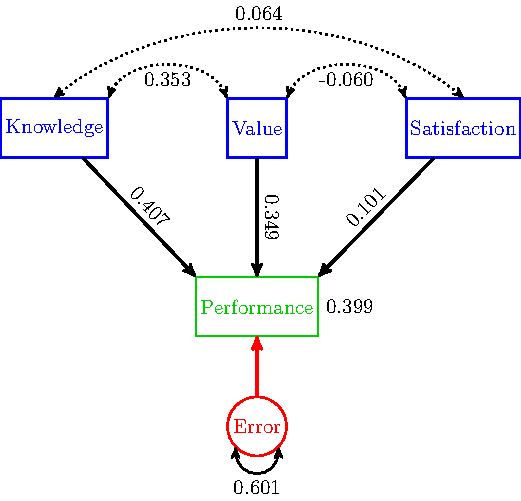
\includegraphics[width=0.8\linewidth]{images/Warren5V1Values} 

}

\caption{Path Diagram with estimates of coefficient for job performance of farm managers}\label{fig:Warren5V1Values}
\end{figure}

\hypertarget{FA}{%
\chapter{Factor Analysis}\label{FA}}

\hypertarget{introduction-3}{%
\section{Introduction}\label{introduction-3}}

The general model for confirmatory factor analysis is

\begin{align}
\mathbf{y}_{i} & =\bm{\Lambda}_{y}\bm{\eta}_{i}+\bm{\epsilon}_{i}\label{eq:MeasurementModel1}\\
\mathbf{x}_{i} & =\bm{\Lambda}_{x}\bm{\xi}_{i}+\bm{\delta}_{i}\label{eq:MeasurementModel2}
\end{align}

The \(\mathbf{y}_{i}\) \(\left(p\times1\right)\) and the \(\mathbf{x}_{i}\)
\(\left(q\times1\right)\) vectors are observed variables, \(\bm{\Lambda}_{y}\)
\(\left(p\times m\right)\) (Lambda) and \(\bm{\Lambda}_{x}\) \(\left(q\times n\right)\)
are the coefficient matrices that show the relation of \(\mathbf{y}_{i}\)
to \(\bm{\eta}_{i}\) and \(\mathbf{x}_{i}\) to \(\bm{\xi}_{i}\) respectively,
and \(\bm{\epsilon}_{i}\) \(\left(p\times1\right)\) (epsilon) and \(\bm{\delta}_{i}\)
\(\left(q\times1\right)\) (delta) are the errors of measurement for
\(\mathbf{y}_{i}\) and \(\mathbf{x}_{i}\), respectively. The errors
of measurement are assumed to be uncorrelated with \(\bm{\eta}_{i}\) and
\(\bm{\xi}_{i}\) and with each other.

\graffito{Aptitude of High School students for Science and Arts}

\begin{figure}[H]

{\centering 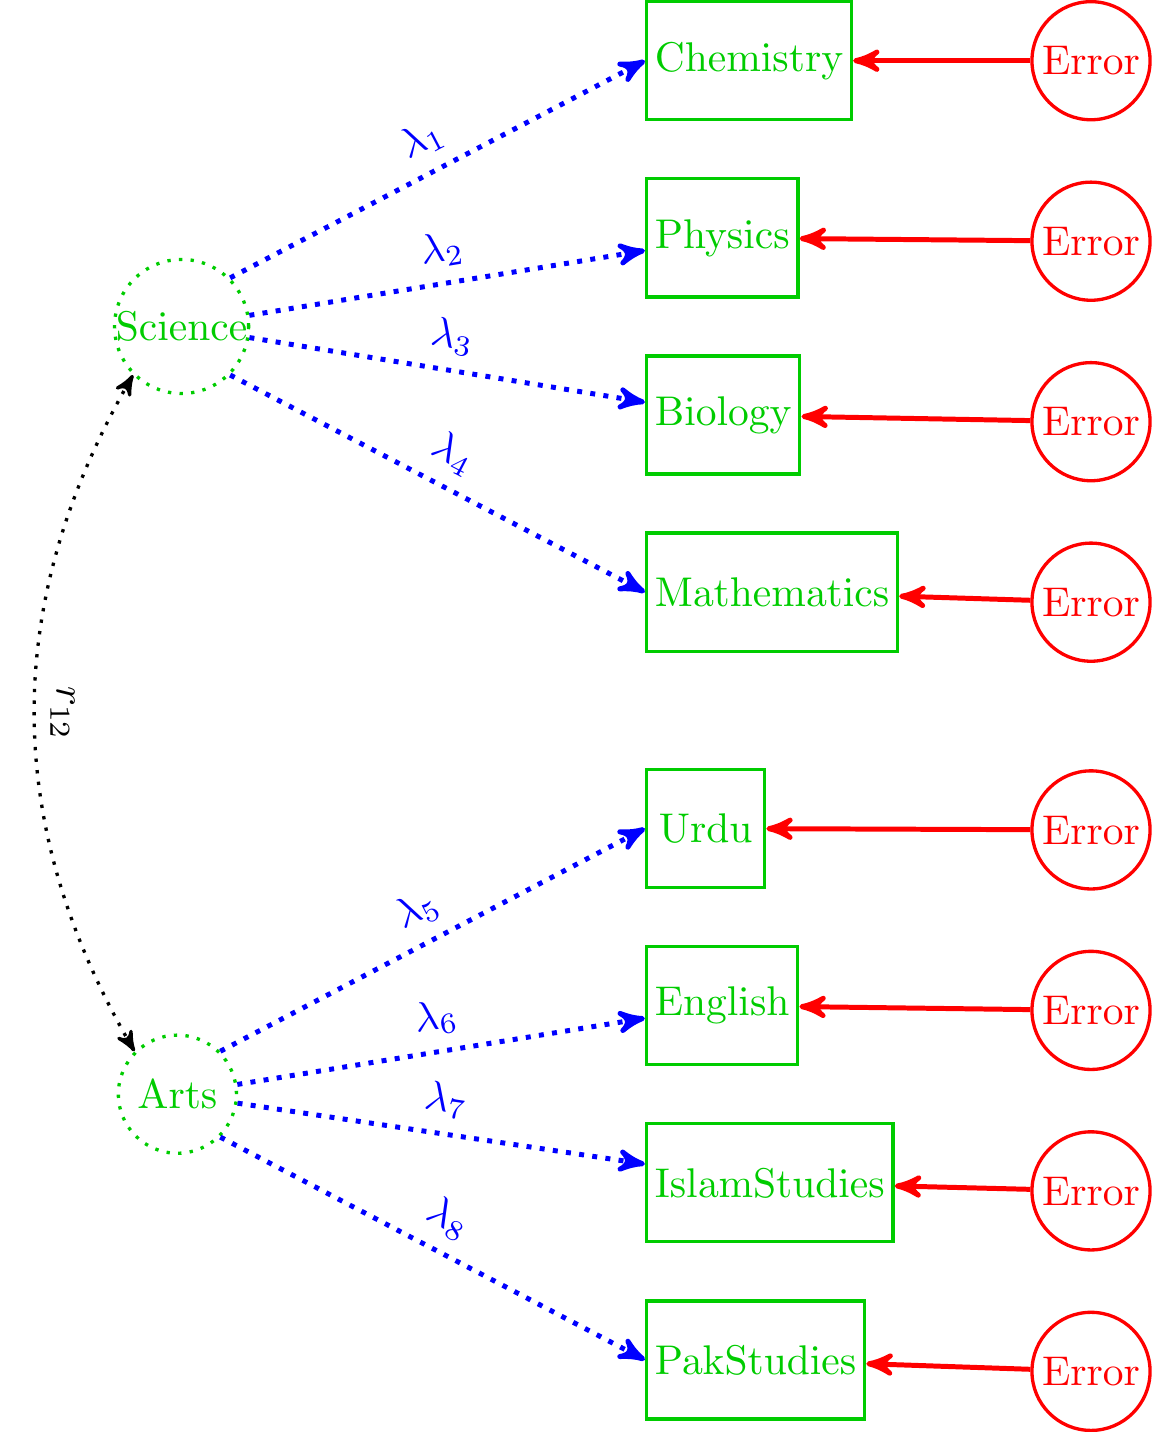
\includegraphics[width=0.8\linewidth]{images/Science1} 

}

\caption{Path Diagram for Aptitude}\label{fig:Science1}
\end{figure}

\begin{example}
Holzinger and Swineford (1939)
\end{example}

\begin{figure}[H]

{\centering 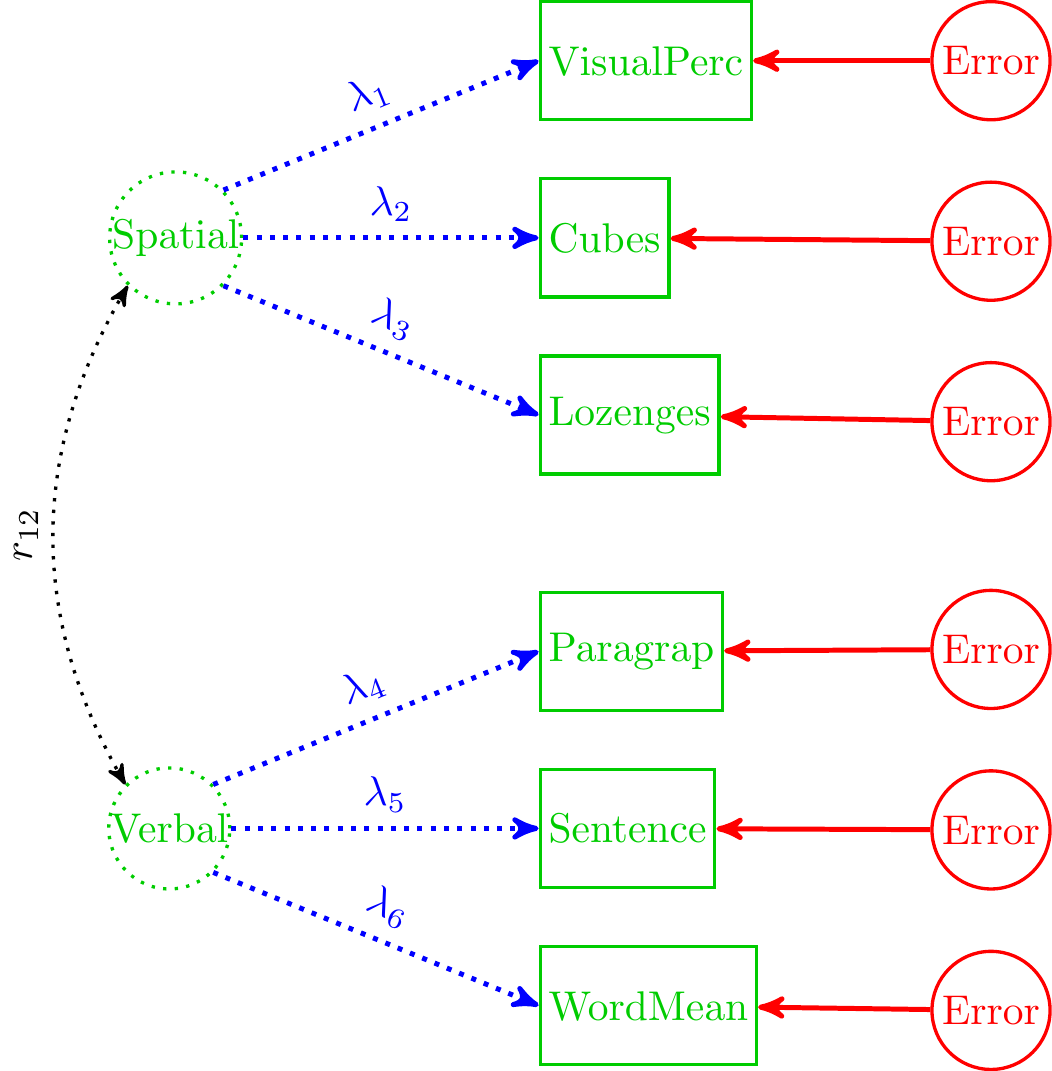
\includegraphics[width=0.8\linewidth]{images/HSF1} 

}

\caption{Path Diagram for Holzinger and Swineford (1939)}\label{fig:HSF1}
\end{figure}

\begin{Shaded}
\begin{Highlighting}[]
\KeywordTok{library}\NormalTok{(lavaan)}

\KeywordTok{load}\NormalTok{(}\StringTok{"HSF.RData"}\NormalTok{)}
\CommentTok{# HSF}
\KeywordTok{str}\NormalTok{(HSF)}
\end{Highlighting}
\end{Shaded}

\begin{verbatim}
'data.frame':   73 obs. of  6 variables:
 $ VisualPerc: num  33 30 36 28 30 20 17 33 30 36 ...
 $ Cubes     : num  22 25 33 25 25 25 21 31 22 28 ...
 $ Lozenges  : num  17 20 36 9 11 6 6 30 20 22 ...
 $ Paragrap  : num  8 10 17 10 11 9 5 11 8 13 ...
 $ Sentence  : num  17 23 25 18 21 21 10 23 17 24 ...
 $ WordMean  : num  10 18 41 11 8 16 10 18 20 36 ...
\end{verbatim}

\begin{Shaded}
\begin{Highlighting}[]
\NormalTok{HSF.sem.m1 <-}\StringTok{ '}
\StringTok{  # Latent Variables}
\StringTok{    Spatial =~ lambda1 * VisualPerc + lambda2 * Cubes +}
\StringTok{               lambda3 * Lozenges}
\StringTok{    Verbal  =~ lambda4 * Paragrap + lambda5 * Sentence +}
\StringTok{               lambda6 * WordMean}

\StringTok{  # Variances and Covariances}
\StringTok{    Spatial  ~~ r12 * Verbal}
\StringTok{'}

\NormalTok{HSF.sem.fm1 <-}
\StringTok{  }\NormalTok{lavaan}\OperatorTok{::}\KeywordTok{sem}\NormalTok{(}
      \DataTypeTok{model            =}\NormalTok{ HSF.sem.m1}
\NormalTok{    , }\DataTypeTok{data             =}\NormalTok{ HSF}
\NormalTok{    , }\DataTypeTok{ordered          =} \OtherTok{NULL}
\NormalTok{    , }\DataTypeTok{sampling.weights =} \OtherTok{NULL}
\NormalTok{    , }\DataTypeTok{sample.cov       =} \OtherTok{NULL}
\NormalTok{    , }\DataTypeTok{sample.mean      =} \OtherTok{NULL}
\NormalTok{    , }\DataTypeTok{sample.nobs      =} \OtherTok{NULL}
\NormalTok{    , }\DataTypeTok{group            =} \OtherTok{NULL}
\NormalTok{    , }\DataTypeTok{cluster          =} \OtherTok{NULL}
  \CommentTok{# , constraints      = ""}
\NormalTok{    , }\DataTypeTok{WLS.V            =} \OtherTok{NULL}
\NormalTok{    , }\DataTypeTok{NACOV            =} \OtherTok{NULL}
  \CommentTok{# ,   ...}
\NormalTok{  )}

\CommentTok{# methods(class = class(HSF.sem.fm1))}
\CommentTok{# anova(HSF.sem.fm1)}
\CommentTok{# coef(HSF.sem.fm1)}
\KeywordTok{parameterEstimates}\NormalTok{(HSF.sem.fm1, }\DataTypeTok{standardized =} \OtherTok{TRUE}\NormalTok{)}
\end{Highlighting}
\end{Shaded}

\begin{verbatim}
          lhs op        rhs   label    est    se     z pvalue
1     Spatial =~ VisualPerc lambda1  1.000 0.000    NA     NA
2     Spatial =~      Cubes lambda2  0.610 0.142 4.279  0.000
3     Spatial =~   Lozenges lambda3  1.198 0.270 4.436  0.000
4      Verbal =~   Paragrap lambda4  1.000 0.000    NA     NA
5      Verbal =~   Sentence lambda5  1.334 0.159 8.379  0.000
6      Verbal =~   WordMean lambda6  2.234 0.262 8.541  0.000
7     Spatial ~~     Verbal     r12  7.315 2.553 2.865  0.004
8  VisualPerc ~~ VisualPerc         23.873 5.945 4.016  0.000
9       Cubes ~~      Cubes         11.602 2.566 4.521  0.000
10   Lozenges ~~   Lozenges         28.275 7.837 3.608  0.000
11   Paragrap ~~   Paragrap          2.834 0.863 3.286  0.001
12   Sentence ~~   Sentence          7.967 1.856 4.292  0.000
13   WordMean ~~   WordMean         19.925 4.917 4.052  0.000
14    Spatial ~~    Spatial         23.302 8.068 2.888  0.004
15     Verbal ~~     Verbal          9.682 2.144 4.516  0.000
   ci.lower ci.upper std.lv std.all std.nox
1     1.000    1.000  4.827   0.703   0.703
2     0.330    0.889  2.943   0.654   0.654
3     0.669    1.728  5.784   0.736   0.736
4     1.000    1.000  3.112   0.880   0.880
5     1.022    1.646  4.151   0.827   0.827
6     1.722    2.747  6.952   0.841   0.841
7     2.311   12.319  0.487   0.487   0.487
8    12.221   35.525 23.873   0.506   0.506
9     6.572   16.631 11.602   0.572   0.572
10   12.914   43.636 28.275   0.458   0.458
11    1.143    4.524  2.834   0.226   0.226
12    4.329   11.605  7.967   0.316   0.316
13   10.288   29.563 19.925   0.292   0.292
14    7.490   39.114  1.000   1.000   1.000
15    5.481   13.884  1.000   1.000   1.000
\end{verbatim}

\begin{Shaded}
\begin{Highlighting}[]
\CommentTok{# fitmeasures(HSF.sem.fm1)}
\KeywordTok{fitted}\NormalTok{(HSF.sem.fm1)}\OperatorTok{$}\NormalTok{cov}
\end{Highlighting}
\end{Shaded}

\begin{verbatim}
           VslPrc Cubes  Lozngs Pargrp Sentnc WordMn
VisualPerc 47.175                                   
Cubes      14.209 20.265                            
Lozenges   27.919 17.024 61.726                     
Paragrap    7.315  4.461  8.765 12.516              
Sentence    9.759  5.950 11.692 12.916 25.197       
WordMean   16.344  9.966 19.583 21.633 28.859 68.260
\end{verbatim}

\begin{Shaded}
\begin{Highlighting}[]
\CommentTok{# residuals(HSF.sem.fm1, type = "cor")}
\CommentTok{# modificationIndices(HSF.sem.fm1)}
\KeywordTok{var}\NormalTok{(HSF)}
\end{Highlighting}
\end{Shaded}

\begin{verbatim}
           VisualPerc     Cubes  Lozenges  Paragrap  Sentence
VisualPerc  47.829909 15.137938 26.899734  8.450723 12.820396
Cubes       15.137938 20.546804 17.658105  3.402207  4.092085
Lozenges    26.899734 17.658105 62.583714  9.181507 13.411339
Paragrap     8.450723  3.402207  9.181507 12.689878 13.042237
Sentence    12.820396  4.092085 13.411339 13.042237 25.546804
WordMean    13.217846  6.934741 24.280061 22.019597 29.245814
            WordMean
VisualPerc 13.217846
Cubes       6.934741
Lozenges   24.280061
Paragrap   22.019597
Sentence   29.245814
WordMean   69.208143
\end{verbatim}

\begin{Shaded}
\begin{Highlighting}[]
\CommentTok{# vcov(HSF.sem.fm1)}


\KeywordTok{summary}\NormalTok{(}
    \DataTypeTok{object       =}\NormalTok{ HSF.sem.fm1}
\NormalTok{  , }\DataTypeTok{header       =} \OtherTok{TRUE}
\NormalTok{  , }\DataTypeTok{fit.measures =} \OtherTok{FALSE}
\NormalTok{  , }\DataTypeTok{estimates    =} \OtherTok{TRUE}
\NormalTok{  , }\DataTypeTok{ci           =} \OtherTok{FALSE}
\NormalTok{  , }\DataTypeTok{fmi          =} \OtherTok{FALSE}
\NormalTok{  , }\DataTypeTok{standardized =} \OtherTok{TRUE}
\NormalTok{  , }\DataTypeTok{rsquare      =} \OtherTok{TRUE}
\NormalTok{  , }\DataTypeTok{std.nox      =} \OtherTok{FALSE}
\NormalTok{  , }\DataTypeTok{modindices   =} \OtherTok{FALSE}
\NormalTok{  , }\DataTypeTok{nd           =}\NormalTok{ 3L}
\NormalTok{)}
\end{Highlighting}
\end{Shaded}

\begin{verbatim}
lavaan 0.6-3 ended normally after 64 iterations

  Optimization method                           NLMINB
  Number of free parameters                         13

  Number of observations                            73

  Estimator                                         ML
  Model Fit Test Statistic                       7.962
  Degrees of freedom                                 8
  P-value (Chi-square)                           0.437

Parameter Estimates:

  Information                                 Expected
  Information saturated (h1) model          Structured
  Standard Errors                             Standard

Latent Variables:
                   Estimate  Std.Err  z-value  P(>|z|)   Std.lv
  Spatial =~                                                   
    VislPrc (lmb1)    1.000                               4.827
    Cubes   (lmb2)    0.610    0.142    4.279    0.000    2.943
    Lozengs (lmb3)    1.198    0.270    4.436    0.000    5.784
  Verbal =~                                                    
    Paragrp (lmb4)    1.000                               3.112
    Sentenc (lmb5)    1.334    0.159    8.379    0.000    4.151
    WordMen (lmb6)    2.234    0.262    8.541    0.000    6.952
  Std.all
         
    0.703
    0.654
    0.736
         
    0.880
    0.827
    0.841

Covariances:
                   Estimate  Std.Err  z-value  P(>|z|)   Std.lv
  Spatial ~~                                                   
    Verbal   (r12)    7.315    2.553    2.865    0.004    0.487
  Std.all
         
    0.487

Variances:
                   Estimate  Std.Err  z-value  P(>|z|)   Std.lv
   .VisualPerc       23.873    5.945    4.016    0.000   23.873
   .Cubes            11.602    2.566    4.521    0.000   11.602
   .Lozenges         28.275    7.837    3.608    0.000   28.275
   .Paragrap          2.834    0.863    3.286    0.001    2.834
   .Sentence          7.967    1.856    4.292    0.000    7.967
   .WordMean         19.925    4.917    4.052    0.000   19.925
    Spatial          23.302    8.068    2.888    0.004    1.000
    Verbal            9.682    2.144    4.516    0.000    1.000
  Std.all
    0.506
    0.572
    0.458
    0.226
    0.316
    0.292
    1.000
    1.000

R-Square:
                   Estimate
    VisualPerc        0.494
    Cubes             0.428
    Lozenges          0.542
    Paragrap          0.774
    Sentence          0.684
    WordMean          0.708
\end{verbatim}

\begin{figure}[H]

{\centering 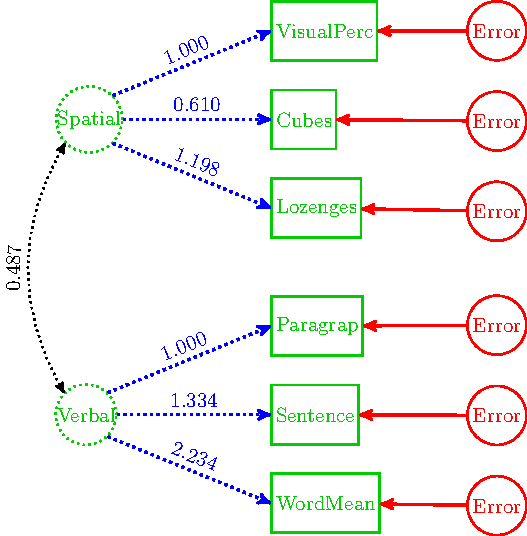
\includegraphics[width=0.8\linewidth]{images/HSF1Values} 

}

\caption{Path Diagram with estimates of coefficients}\label{fig:HSF1Values}
\end{figure}

\hypertarget{SEM}{%
\chapter{Strucural Equation Modeling with Latent Variables}\label{SEM}}

\hypertarget{introduction-4}{%
\section{Introduction}\label{introduction-4}}

\graffito{General Structural Equation Model}

The \emph{general structural equation model} consists of a \emph{measurement model} that specifies the relation of observed to latent variables and a \emph{latent variable model} that
shows the influence of latent variables on each other.

The first component of the structural equations is the latent variable model:

\graffito{Latent Variable Model}

\begin{equation}
\bm{\eta}_{i}=\mathbf{B}\bm{\eta}_{i}+\bm{\Gamma}\bm{\xi}_{i}+\bm{\zeta}_{i}\label{eq:StructuralModel2}
\end{equation}

In \eqref{eq:StructuralModel2}, \(\bm{\eta}_{i}\) (eta), the vector
of latent endogenous random variables, is \(m\times1\); \(\bm{\xi}_{i}\)
(xi) the latent exogenous random variables, is \(n\times1\); \(\mathbf{B}\)
is the \(m\times m\) coefficient matrix showing the influence of the
latent endogenous variables on each other; \(\bm{\Gamma}\) (Gamma)
is the \(m\times n\) coefficient matrix for the effects of \(\bm{\xi}_{i}\)
on \(\bm{\eta}_{i}\). The matrix \(\left(\mathbf{I}-\mathbf{B}\right)\)
is non-singular. \(\bm{\zeta}_{i}\) (zeta) is the disturbance vector
that is assumed to have an expected value of zero \(\left[\mathbb{E}\left(\bm{\zeta}_{i}\right)=\mathbf{0}\right]\)
and which is uncorrelated with \(\bm{\xi}_{i}\).

The second component of the general system is the measurement model:

\graffito{Measurement Model}

\begin{align}
\mathbf{y}_{i} & =\bm{\Lambda}_{y}\bm{\eta}_{i}+\bm{\epsilon}_{i}\label{eq:MeasurementModel1}\\
\mathbf{x}_{i} & =\bm{\Lambda}_{x}\bm{\xi}_{i}+\bm{\delta}_{i}\label{eq:MeasurementModel2}
\end{align}

The \(\mathbf{y}_{i}\) \(\left(p\times1\right)\) and the \(\mathbf{x}_{i}\)
\(\left(q\times1\right)\) vectors are observed variables, \(\bm{\Lambda}_{y}\)
\(\left(p\times m\right)\) (Lambda) and \(\bm{\Lambda}_{x}\) \(\left(q\times n\right)\)
are the coefficient matrices that show the relation of \(\mathbf{y}_{i}\)
to \(\bm{\eta}_{i}\) and \(\mathbf{x}_{i}\) to \(\bm{\xi}_{i}\) respectively,
and \(\bm{\epsilon}_{i}\) \(\left(p\times1\right)\) (epsilon) and \(\bm{\delta}_{i}\)
\(\left(q\times1\right)\) (delta) are the errors of measurement for
\(\mathbf{y}_{i}\) and \(\mathbf{x}_{i}\), respectively. The errors
of measurement are assumed to be uncorrelated with \(\bm{\eta}_{i}\),
\(\bm{\xi}_{i}\) and \(\bm{\zeta}_{i}\) and with each other.

Also \(\mathbb{V}\left(\bm{\xi}_{i}\right)=\bm{\Phi}\) (Phi), \(\mathbb{V}\left(\bm{\zeta}_{i}\right)=\bm{\Psi}\)
(Psi), \(\mathbb{V}\left(\bm{\epsilon}_{i}\right)=\bm{\Theta}_{\epsilon}\)
(Theta), \(\mathbb{V}\left(\bm{\delta}_{i}\right)=\bm{\Theta}_{\delta}\)
(Theta) and \(\mathbb{V}\left(\begin{bmatrix}\mathbf{y}_{i}\\ \mathbf{x}_{i} \end{bmatrix}\right)=\bm{\Sigma}\) (Sigma).

\begin{figure}[H]

{\centering 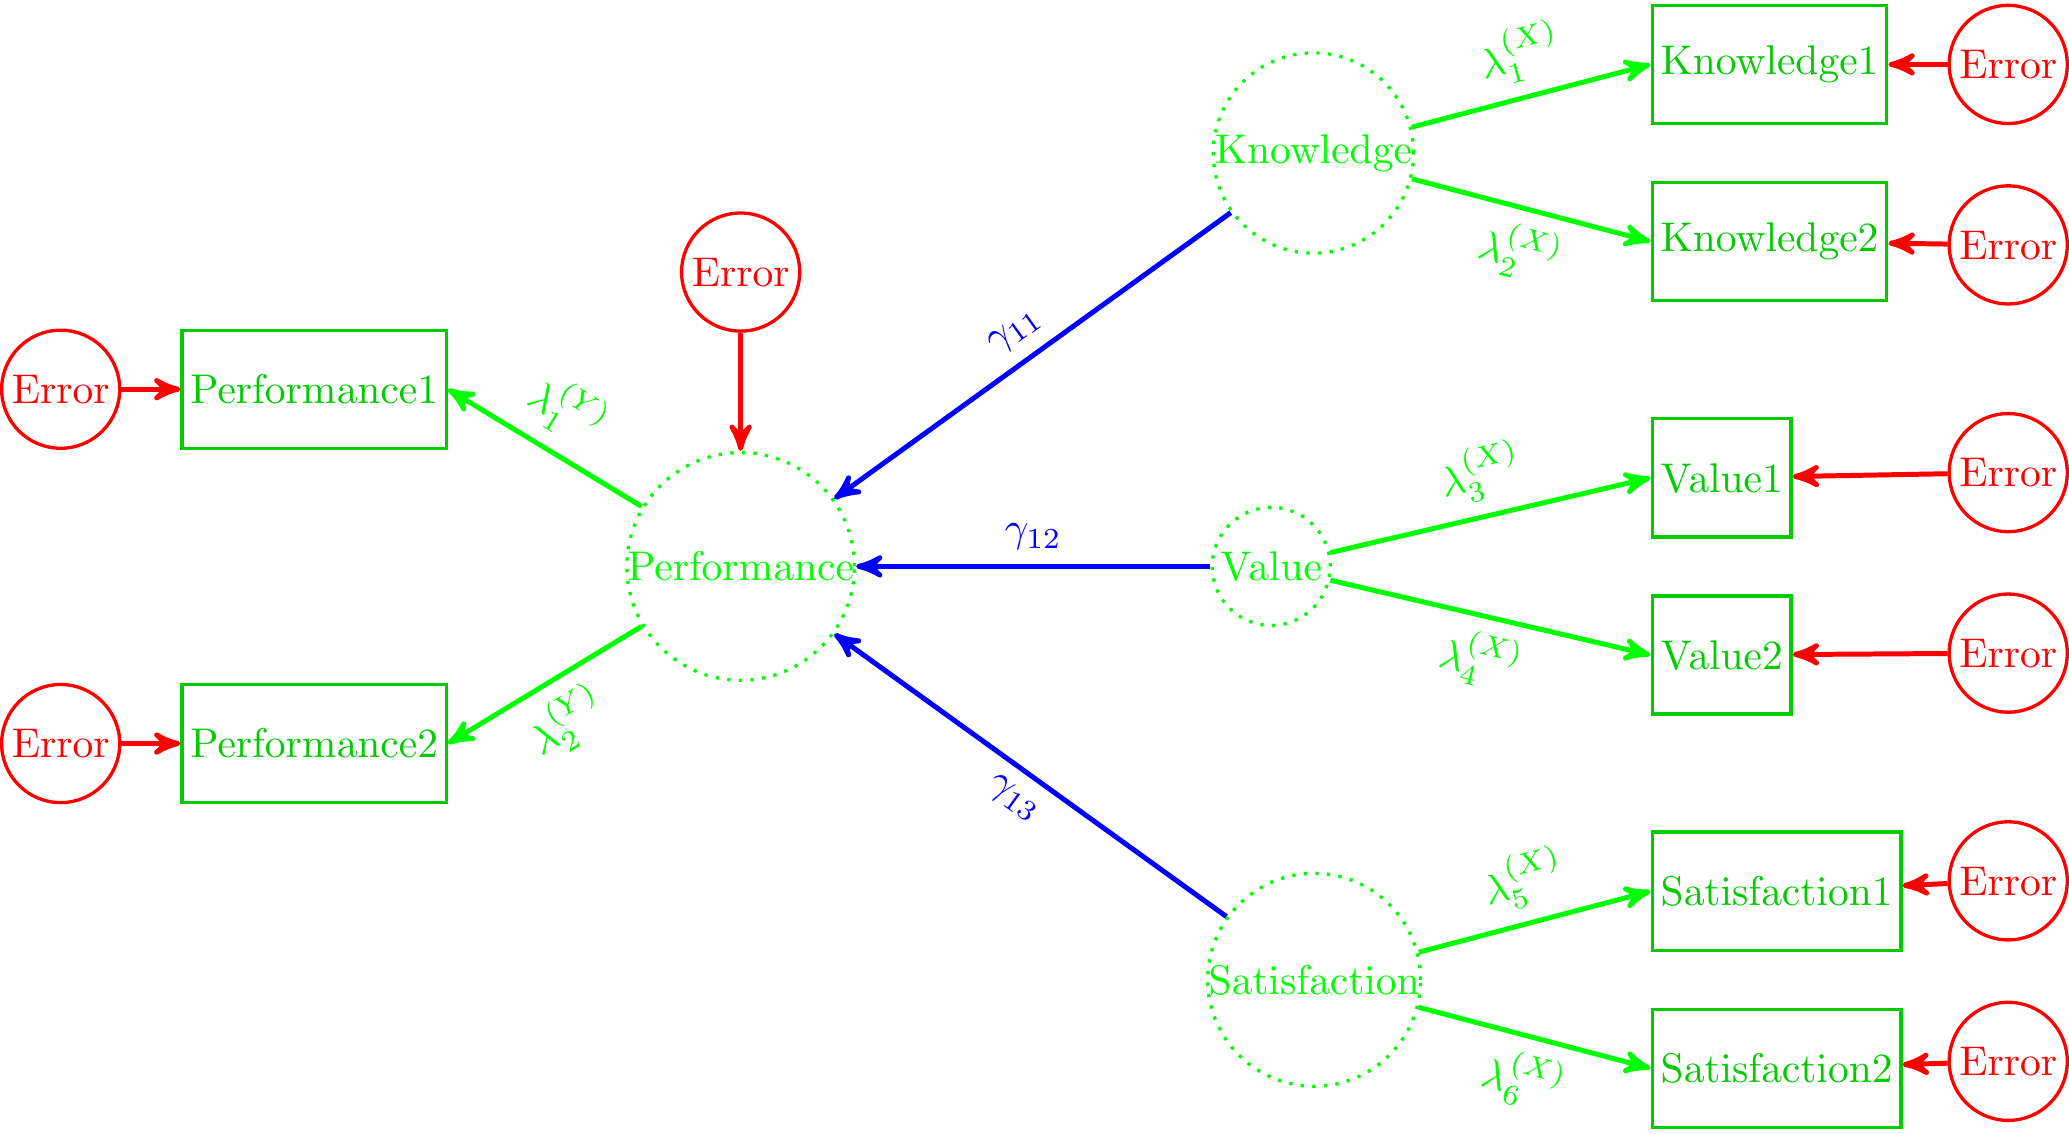
\includegraphics[width=0.8\linewidth]{images/Warren8V1} 

}

\caption{Path Diagram for job performance of farm managers}\label{fig:Warren8V1}
\end{figure}

\begin{Shaded}
\begin{Highlighting}[]
\KeywordTok{library}\NormalTok{(lavaan)}

\NormalTok{Warren8V <-}
\StringTok{  }\KeywordTok{matrix}\NormalTok{(}
    \DataTypeTok{data =}
\KeywordTok{c}\NormalTok{(}
\FloatTok{0.0271}\NormalTok{, }\FloatTok{0.0172}\NormalTok{,  }\FloatTok{0.0219}\NormalTok{, }\FloatTok{0.0164}\NormalTok{,  }\FloatTok{0.0284}\NormalTok{,  }\FloatTok{0.0217}\NormalTok{,  }\FloatTok{0.0083}\NormalTok{,  }\FloatTok{0.0074}\NormalTok{,}
\FloatTok{0.0172}\NormalTok{, }\FloatTok{0.0222}\NormalTok{,  }\FloatTok{0.0193}\NormalTok{, }\FloatTok{0.0130}\NormalTok{,  }\FloatTok{0.0294}\NormalTok{,  }\FloatTok{0.0185}\NormalTok{,  }\FloatTok{0.0011}\NormalTok{,  }\FloatTok{0.0015}\NormalTok{,}
\FloatTok{0.0219}\NormalTok{, }\FloatTok{0.0193}\NormalTok{,  }\FloatTok{0.0876}\NormalTok{, }\FloatTok{0.0317}\NormalTok{,  }\FloatTok{0.0383}\NormalTok{,  }\FloatTok{0.0356}\NormalTok{, }\FloatTok{-0.0001}\NormalTok{,  }\FloatTok{0.0035}\NormalTok{,}
\FloatTok{0.0164}\NormalTok{, }\FloatTok{0.0130}\NormalTok{,  }\FloatTok{0.0317}\NormalTok{, }\FloatTok{0.0568}\NormalTok{,  }\FloatTok{0.0151}\NormalTok{,  }\FloatTok{0.0230}\NormalTok{,  }\FloatTok{0.0055}\NormalTok{,  }\FloatTok{0.0089}\NormalTok{,}
\FloatTok{0.0284}\NormalTok{, }\FloatTok{0.0294}\NormalTok{,  }\FloatTok{0.0383}\NormalTok{, }\FloatTok{0.0151}\NormalTok{,  }\FloatTok{0.1826}\NormalTok{,  }\FloatTok{0.0774}\NormalTok{, }\FloatTok{-0.0087}\NormalTok{, }\FloatTok{-0.0007}\NormalTok{,}
\FloatTok{0.0217}\NormalTok{, }\FloatTok{0.0185}\NormalTok{,  }\FloatTok{0.0356}\NormalTok{, }\FloatTok{0.0230}\NormalTok{,  }\FloatTok{0.0774}\NormalTok{,  }\FloatTok{0.1473}\NormalTok{, }\FloatTok{-0.0069}\NormalTok{, }\FloatTok{-0.0088}\NormalTok{,}
\FloatTok{0.0083}\NormalTok{, }\FloatTok{0.0011}\NormalTok{, }\FloatTok{-0.0001}\NormalTok{, }\FloatTok{0.0055}\NormalTok{, }\FloatTok{-0.0087}\NormalTok{, }\FloatTok{-0.0069}\NormalTok{,  }\FloatTok{0.1137}\NormalTok{,  }\FloatTok{0.0722}\NormalTok{,}
\FloatTok{0.0074}\NormalTok{, }\FloatTok{0.0015}\NormalTok{,  }\FloatTok{0.0035}\NormalTok{, }\FloatTok{0.0089}\NormalTok{, }\FloatTok{-0.0007}\NormalTok{, }\FloatTok{-0.0088}\NormalTok{,  }\FloatTok{0.0722}\NormalTok{,  }\FloatTok{0.1024}
\NormalTok{)}
\NormalTok{    , }\DataTypeTok{nrow  =} \DecValTok{8}
\NormalTok{    , }\DataTypeTok{ncol  =} \DecValTok{8}
\NormalTok{    , }\DataTypeTok{byrow =} \OtherTok{TRUE}
\NormalTok{    , }\DataTypeTok{dimnames =} \KeywordTok{list}\NormalTok{(}\KeywordTok{c}\NormalTok{(}\StringTok{"Performance1"}\NormalTok{, }\StringTok{"Performance2"}\NormalTok{,}
                        \StringTok{"Knowledge1"}\NormalTok{,   }\StringTok{"Knowledge2"}\NormalTok{,}
                        \StringTok{"Value1"}\NormalTok{,   }\StringTok{"Value2"}\NormalTok{,}
                        \StringTok{"Satisfaction1"}\NormalTok{, }\StringTok{"Satisfaction2"}\NormalTok{)}
\NormalTok{                      , }\KeywordTok{c}\NormalTok{(}\StringTok{"Performance1"}\NormalTok{,   }\StringTok{"Performance2"}\NormalTok{,}
                          \StringTok{"Knowledge1"}\NormalTok{, }\StringTok{"Knowledge2"}\NormalTok{,}
                          \StringTok{"Value1"}\NormalTok{, }\StringTok{"Value2"}\NormalTok{,}
                          \StringTok{"Satisfaction1"}\NormalTok{, }\StringTok{"Satisfaction2"}\NormalTok{)}
\NormalTok{    )}

\NormalTok{  )}

\NormalTok{Warren8V}
\end{Highlighting}
\end{Shaded}

\begin{verbatim}
              Performance1 Performance2 Knowledge1 Knowledge2
Performance1        0.0271       0.0172     0.0219     0.0164
Performance2        0.0172       0.0222     0.0193     0.0130
Knowledge1          0.0219       0.0193     0.0876     0.0317
Knowledge2          0.0164       0.0130     0.0317     0.0568
Value1              0.0284       0.0294     0.0383     0.0151
Value2              0.0217       0.0185     0.0356     0.0230
Satisfaction1       0.0083       0.0011    -0.0001     0.0055
Satisfaction2       0.0074       0.0015     0.0035     0.0089
               Value1  Value2 Satisfaction1 Satisfaction2
Performance1   0.0284  0.0217        0.0083        0.0074
Performance2   0.0294  0.0185        0.0011        0.0015
Knowledge1     0.0383  0.0356       -0.0001        0.0035
Knowledge2     0.0151  0.0230        0.0055        0.0089
Value1         0.1826  0.0774       -0.0087       -0.0007
Value2         0.0774  0.1473       -0.0069       -0.0088
Satisfaction1 -0.0087 -0.0069        0.1137        0.0722
Satisfaction2 -0.0007 -0.0088        0.0722        0.1024
\end{verbatim}

\begin{Shaded}
\begin{Highlighting}[]
\NormalTok{Warren8V.sem.m1 <-}\StringTok{ '}
\StringTok{  # Latent Variables}
\StringTok{    Performance  =~ lambda1Y * Performance1 + lambda2Y * Performance2}
\StringTok{    Knowledge    =~ lambda1X * Knowledge1 + lambda2X * Knowledge2}
\StringTok{    Value        =~ lambda3X * Value1 + lambda4X * Value2}
\StringTok{    Satisfaction =~ lambda5X * Satisfaction1 + lambda6X * Satisfaction2}

\StringTok{  # Regressions}
\StringTok{    Performance ~ gamma11 * Knowledge + gamma12 *Value +}
\StringTok{                  gamma13 *Satisfaction}

\StringTok{  # Variances and Covariances}
\StringTok{    Knowledge   ~~ r12 * Value}
\StringTok{    Knowledge   ~~ r13 * Satisfaction}
\StringTok{    Value       ~~ r23 * Satisfaction}
\StringTok{    Performance ~~ sigma2P * Performance}
\StringTok{'}

\NormalTok{Warren8V.sem.fm1 <-}
\StringTok{  }\NormalTok{lavaan}\OperatorTok{::}\KeywordTok{sem}\NormalTok{(}
      \DataTypeTok{model            =}\NormalTok{ Warren8V.sem.m1}
  \CommentTok{# , data}
\NormalTok{    , }\DataTypeTok{ordered          =} \OtherTok{NULL}
\NormalTok{    , }\DataTypeTok{sampling.weights =} \OtherTok{NULL}
\NormalTok{    , }\DataTypeTok{sample.cov       =}\NormalTok{ Warren8V}
\NormalTok{    , }\DataTypeTok{sample.mean      =} \OtherTok{NULL}
\NormalTok{    , }\DataTypeTok{sample.nobs      =} \DecValTok{98}
\NormalTok{    , }\DataTypeTok{group            =} \OtherTok{NULL}
\NormalTok{    , }\DataTypeTok{cluster          =} \OtherTok{NULL}
  \CommentTok{# , constraints      = ""}
\NormalTok{    , }\DataTypeTok{WLS.V            =} \OtherTok{NULL}
\NormalTok{    , }\DataTypeTok{NACOV            =} \OtherTok{NULL}
  \CommentTok{# ,   ...}
\NormalTok{  )}

\CommentTok{# methods(class = class(Warren8V.sem.fm1))}
\CommentTok{# anova(Warren8V.sem.fm1)}
\CommentTok{# coef(Warren8V.sem.fm1)}
\KeywordTok{parameterEstimates}\NormalTok{(Warren8V.sem.fm1, }\DataTypeTok{standardized =} \OtherTok{TRUE}\NormalTok{)}
\end{Highlighting}
\end{Shaded}

\begin{verbatim}
             lhs op           rhs    label    est    se      z
1    Performance =~  Performance1 lambda1Y  1.000 0.000     NA
2    Performance =~  Performance2 lambda2Y  0.867 0.116  7.489
3      Knowledge =~    Knowledge1 lambda1X  1.000 0.000     NA
4      Knowledge =~    Knowledge2 lambda2X  0.683 0.160  4.274
5          Value =~        Value1 lambda3X  1.000 0.000     NA
6          Value =~        Value2 lambda4X  0.763 0.184  4.149
7   Satisfaction =~ Satisfaction1 lambda5X  1.000 0.000     NA
8   Satisfaction =~ Satisfaction2 lambda6X  0.792 0.436  1.816
9    Performance  ~     Knowledge  gamma11  0.337 0.124  2.711
10   Performance  ~         Value  gamma12  0.176 0.079  2.237
11   Performance  ~  Satisfaction  gamma13  0.061 0.054  1.132
12     Knowledge ~~         Value      r12  0.037 0.012  3.052
13     Knowledge ~~  Satisfaction      r13  0.004 0.009  0.464
14         Value ~~  Satisfaction      r23 -0.008 0.013 -0.614
15   Performance ~~   Performance  sigma2P  0.007 0.003  2.590
16  Performance1 ~~  Performance1           0.007 0.002  3.126
17  Performance2 ~~  Performance2           0.007 0.002  3.891
18    Knowledge1 ~~    Knowledge1           0.041 0.011  3.629
19    Knowledge2 ~~    Knowledge2           0.035 0.007  5.193
20        Value1 ~~        Value1           0.080 0.025  3.266
21        Value2 ~~        Value2           0.087 0.018  4.916
22 Satisfaction1 ~~ Satisfaction1           0.022 0.049  0.453
23 Satisfaction2 ~~ Satisfaction2           0.045 0.031  1.428
24     Knowledge ~~     Knowledge           0.046 0.015  3.154
25         Value ~~         Value           0.100 0.032  3.164
26  Satisfaction ~~  Satisfaction           0.090 0.051  1.754
   pvalue ci.lower ci.upper std.lv std.all std.nox
1      NA    1.000    1.000  0.140   0.856   0.856
2   0.000    0.640    1.093  0.121   0.819   0.819
3      NA    1.000    1.000  0.214   0.728   0.728
4   0.000    0.370    0.997  0.146   0.618   0.618
5      NA    1.000    1.000  0.317   0.745   0.745
6   0.000    0.402    1.123  0.242   0.633   0.633
7      NA    1.000    1.000  0.300   0.896   0.896
8   0.069   -0.063    1.646  0.238   0.747   0.747
9   0.007    0.093    0.581  0.516   0.516   0.516
10  0.025    0.022    0.330  0.398   0.398   0.398
11  0.257   -0.044    0.166  0.130   0.130   0.130
12  0.002    0.013    0.060  0.542   0.542   0.542
13  0.643   -0.013    0.022  0.064   0.064   0.064
14  0.539   -0.033    0.018 -0.084  -0.084  -0.084
15  0.010    0.002    0.012  0.337   0.337   0.337
16  0.002    0.003    0.012  0.007   0.268   0.268
17  0.000    0.004    0.011  0.007   0.329   0.329
18  0.000    0.019    0.063  0.041   0.471   0.471
19  0.000    0.022    0.048  0.035   0.619   0.619
20  0.001    0.032    0.128  0.080   0.444   0.444
21  0.000    0.053    0.122  0.087   0.599   0.599
22  0.650   -0.074    0.119  0.022   0.198   0.198
23  0.153   -0.017    0.106  0.045   0.442   0.442
24  0.002    0.017    0.074  1.000   1.000   1.000
25  0.002    0.038    0.163  1.000   1.000   1.000
26  0.080   -0.011    0.191  1.000   1.000   1.000
\end{verbatim}

\begin{Shaded}
\begin{Highlighting}[]
\CommentTok{# fitmeasures(Warren8V.sem.fm1)}
\KeywordTok{fitted}\NormalTok{(Warren8V.sem.fm1)}\OperatorTok{$}\NormalTok{cov}
\end{Highlighting}
\end{Shaded}

\begin{verbatim}
              Prfrm1 Prfrm2 Knwld1 Knwld2 Value1 Value2 Stsfc1
Performance1   0.027                                          
Performance2   0.017  0.022                                   
Knowledge1     0.022  0.019  0.087                            
Knowledge2     0.015  0.013  0.031  0.056                     
Value1         0.030  0.026  0.037  0.025  0.181              
Value2         0.023  0.020  0.028  0.019  0.077  0.146       
Satisfaction1  0.005  0.005  0.004  0.003 -0.008 -0.006  0.113
Satisfaction2  0.004  0.004  0.003  0.002 -0.006 -0.005  0.071
              Stsfc2
Performance1        
Performance2        
Knowledge1          
Knowledge2          
Value1              
Value2              
Satisfaction1       
Satisfaction2  0.101
\end{verbatim}

\begin{Shaded}
\begin{Highlighting}[]
\CommentTok{# residuals(Warren8V.sem.fm1, type = "cor")}
\CommentTok{# modificationIndices(Warren8V.sem.fm1)}
\NormalTok{Warren8V}
\end{Highlighting}
\end{Shaded}

\begin{verbatim}
              Performance1 Performance2 Knowledge1 Knowledge2
Performance1        0.0271       0.0172     0.0219     0.0164
Performance2        0.0172       0.0222     0.0193     0.0130
Knowledge1          0.0219       0.0193     0.0876     0.0317
Knowledge2          0.0164       0.0130     0.0317     0.0568
Value1              0.0284       0.0294     0.0383     0.0151
Value2              0.0217       0.0185     0.0356     0.0230
Satisfaction1       0.0083       0.0011    -0.0001     0.0055
Satisfaction2       0.0074       0.0015     0.0035     0.0089
               Value1  Value2 Satisfaction1 Satisfaction2
Performance1   0.0284  0.0217        0.0083        0.0074
Performance2   0.0294  0.0185        0.0011        0.0015
Knowledge1     0.0383  0.0356       -0.0001        0.0035
Knowledge2     0.0151  0.0230        0.0055        0.0089
Value1         0.1826  0.0774       -0.0087       -0.0007
Value2         0.0774  0.1473       -0.0069       -0.0088
Satisfaction1 -0.0087 -0.0069        0.1137        0.0722
Satisfaction2 -0.0007 -0.0088        0.0722        0.1024
\end{verbatim}

\begin{Shaded}
\begin{Highlighting}[]
\CommentTok{# vcov(Warren8V.sem.fm1)}



\KeywordTok{summary}\NormalTok{(}
    \DataTypeTok{object       =}\NormalTok{ Warren8V.sem.fm1}
\NormalTok{  , }\DataTypeTok{header       =} \OtherTok{TRUE}
\NormalTok{  , }\DataTypeTok{fit.measures =} \OtherTok{FALSE}
\NormalTok{  , }\DataTypeTok{estimates    =} \OtherTok{TRUE}
\NormalTok{  , }\DataTypeTok{ci           =} \OtherTok{FALSE}
\NormalTok{  , }\DataTypeTok{fmi          =} \OtherTok{FALSE}
\NormalTok{  , }\DataTypeTok{standardized =} \OtherTok{TRUE}
\NormalTok{  , }\DataTypeTok{rsquare      =} \OtherTok{TRUE}
\NormalTok{  , }\DataTypeTok{std.nox      =} \OtherTok{FALSE}
\NormalTok{  , }\DataTypeTok{modindices   =} \OtherTok{FALSE}
\NormalTok{  , }\DataTypeTok{nd           =}\NormalTok{ 3L}
\NormalTok{)}
\end{Highlighting}
\end{Shaded}

\begin{verbatim}
lavaan 0.6-3 ended normally after 75 iterations

  Optimization method                           NLMINB
  Number of free parameters                         22

  Number of observations                            98

  Estimator                                         ML
  Model Fit Test Statistic                      10.441
  Degrees of freedom                                14
  P-value (Chi-square)                           0.729

Parameter Estimates:

  Information                                 Expected
  Information saturated (h1) model          Structured
  Standard Errors                             Standard

Latent Variables:
                   Estimate  Std.Err  z-value  P(>|z|)   Std.lv
  Performance =~                                               
    Prfrmn1 (lm1Y)    1.000                               0.140
    Prfrmn2 (lm2Y)    0.867    0.116    7.489    0.000    0.121
  Knowledge =~                                                 
    Knwldg1 (lm1X)    1.000                               0.214
    Knwldg2 (lm2X)    0.683    0.160    4.274    0.000    0.146
  Value =~                                                     
    Value1  (lm3X)    1.000                               0.317
    Value2  (lm4X)    0.763    0.184    4.149    0.000    0.242
  Satisfaction =~                                              
    Stsfct1 (lm5X)    1.000                               0.300
    Stsfct2 (lm6X)    0.792    0.436    1.816    0.069    0.238
  Std.all
         
    0.856
    0.819
         
    0.728
    0.618
         
    0.745
    0.633
         
    0.896
    0.747

Regressions:
                   Estimate  Std.Err  z-value  P(>|z|)   Std.lv
  Performance ~                                                
    Knowldg (gm11)    0.337    0.124    2.711    0.007    0.516
    Value   (gm12)    0.176    0.079    2.237    0.025    0.398
    Stsfctn (gm13)    0.061    0.054    1.132    0.257    0.130
  Std.all
         
    0.516
    0.398
    0.130

Covariances:
                   Estimate  Std.Err  z-value  P(>|z|)   Std.lv
  Knowledge ~~                                                 
    Value    (r12)    0.037    0.012    3.052    0.002    0.542
    Satsfctn (r13)    0.004    0.009    0.464    0.643    0.064
  Value ~~                                                     
    Satsfctn (r23)   -0.008    0.013   -0.614    0.539   -0.084
  Std.all
         
    0.542
    0.064
         
   -0.084

Variances:
                   Estimate  Std.Err  z-value  P(>|z|)   Std.lv
   .Prfrmnc (sg2P)    0.007    0.003    2.590    0.010    0.337
   .Prfrmn1           0.007    0.002    3.126    0.002    0.007
   .Prfrmn2           0.007    0.002    3.891    0.000    0.007
   .Knwldg1           0.041    0.011    3.629    0.000    0.041
   .Knwldg2           0.035    0.007    5.193    0.000    0.035
   .Value1            0.080    0.025    3.266    0.001    0.080
   .Value2            0.087    0.018    4.916    0.000    0.087
   .Stsfct1           0.022    0.049    0.453    0.650    0.022
   .Stsfct2           0.045    0.031    1.428    0.153    0.045
    Knowldg           0.046    0.015    3.154    0.002    1.000
    Value             0.100    0.032    3.164    0.002    1.000
    Stsfctn           0.090    0.051    1.754    0.080    1.000
  Std.all
    0.337
    0.268
    0.329
    0.471
    0.619
    0.444
    0.599
    0.198
    0.442
    1.000
    1.000
    1.000

R-Square:
                   Estimate
    Performance       0.663
    Performance1      0.732
    Performance2      0.671
    Knowledge1        0.529
    Knowledge2        0.381
    Value1            0.556
    Value2            0.401
    Satisfaction1     0.802
    Satisfaction2     0.558
\end{verbatim}

% Bibliography

\label{app:bibliography} % Reference the bibliography elsewhere with \autoref{app:bibliography}

\manualmark
\markboth{\textsc{\bibname}}{\textsc{\bibname}}
\refstepcounter{dummy}

\addtocontents{toc}{\protect\vspace{\beforebibskip}} % Place the bibliography slightly below the rest of the document content in the table of contents


\bibliographystyle{plainnat}

\nocite{*}

%\bibliography{bib/bib}
\bibliography{bib/SEM.bib}

%\end{CJK*}
\end{document}
